        %%******************************************%%
        %%                                          %%
        %%        Modello di tesi di laurea         %%
        %%            di Andrea Giraldin            %%
        %%                                          %%
        %%             2 novembre 2012              %%
        %%                                          %%
        %%******************************************%%

\begin{document}
    \frontmatter
    \begin{titlepage}
    \begin{center}
        \begin{LARGE}
            \textbf{\myUni}\\
        \end{LARGE}

        \vspace{10pt}

        \begin{Large}
            \textsc{\myDepartment}\\
        \end{Large}

        \vspace{10pt}

        \begin{large}
            \textsc{\myFaculty}\\
        \end{large}

        \vspace{30pt}
        \begin{figure}[htbp]
            \centering
            
\includegraphics[height=6cm]{unipd-logo}
        \end{figure}
        \vspace{30pt}

        \begin{LARGE}
            \textbf{\myTitle}\\
        \end{LARGE}

        \vspace{10pt}

        \begin{large}
            \textsl{\myDegree}\\
        \end{large}

        \vspace{40pt}

        \begin{large}
            \begin{flushleft}
                \textit{Relatore}\\
                \vspace{5pt}
                \profTitle\ \myProf
            \end{flushleft}

            % You can tweak the spacing to have professor and student names on the same line
            % useful if the page is broken by a long thesis title and you need more space
            % \vspace{-52pt}

            \begin{flushright}
                \textit{Laureando}\\
                \vspace{5pt}
                \myName
            \end{flushright}
        \end{large}

        \vspace{40pt}

        \line(1, 0){338} \\
        \begin{normalsize}
            \textsc{Anno Accademico \myAA}
        \end{normalsize}
    \end{center}
\end{titlepage}

    \clearpage
\phantomsection
\thispagestyle{empty}

\hfill
\vfill

\noindent\myName: \textit{\myTitle,}
\myDegree,
\textcopyright\ \myTime.

    %\cleardoublepage
\phantomsection
\thispagestyle{empty}
\pdfbookmark{Dedica}{Dedica}

\vspace*{3cm}

\begin{center}
    Lorem ipsum dolor sit amet, consectetuer adipiscing elit. \\ \medskip
    --- Oscar Wilde
\end{center}

\medskip

\begin{center}
    Dedicato a ...
\end{center}

    \cleardoublepage
\phantomsection
\pdfbookmark{Sommario}{Sommario}
\begingroup
\let\clearpage\relax
\let\cleardoublepage\relax
\let\cleardoublepage\relax

\chapter*{Sommario}

Il presente documento espone il lavoro svolto dal laureando Nicola Baesso, presso l'azienda ESignWorld S.R.L., durante il tirocinio della durata di circa trecento ore.\\\\
Il tirocinio prevedeva inanzitutto lo sviluppo di un applicativo \emph{desktop} da utilizzare in un \emph{device} di firma, unendo tecnologie \emph{front-end} e \emph{back-end}.\\
In particolare, era richiesto lo sviluppo dell'applicazione, utilizzando \emph{Electron} e il \emph{framework} \emph{Angular}.\\
Inoltre, volendo recuperare i dati dal \emph{device} di firma, l'applicazione necessitava l'utilizzo di moduli compilati per \emph{NodeJS}, e scritti in \emph{C++}.\\\\
Lo scopo di tale progetto era dimostrare che il \emph{device} utilizzato non si limitasse alla semplice firma, ma che potesse essere un ottimo strumento multimediale, in particolare un ottimo strumento per l'utilizzo di \emph{videogames}.\\

%\vfill

%\selectlanguage{english}
%\pdfbookmark{Abstract}{Abstract}
%\chapter*{Abstract}

%\selectlanguage{italian}

\endgroup

\vfill

    \cleardoublepage
\phantomsection
\pdfbookmark{Ringraziamenti}{ringraziamenti}


\bigskip

\begingroup
\let\clearpage\relax
\let\cleardoublepage\relax
\let\cleardoublepage\relax

\chapter*{Ringraziamenti}

\textit{Innanzitutto, vorrei esprimere la mia gratitudine al Prof. \myProf, relatore della mia tesi, per l'aiuto e il sostegno fornitomi durante la stesura del lavoro.}\\
\textit{Inoltre, ringrazio profondamente il signor \myTutor, mio tutor aziendale, per avermi affiancato durante il lavoro.}\\
\textit{Desidero ringraziare con affetto i miei genitori e la mia ragazza, per il sostegno e per essermi stati vicini in ogni momento durante gli anni di studio.}\\
\textit{Desiderio ringraziare anche i miei amici, sia quelli conosciuti durante il mio percorso sia chi conoscevo già da prima, per tutti i momenti passati insieme.}\\
\textit{Infine, ringrazio anche chi, senza tanti complimenti, si è allontanato dalla mia vita durante questi anni. Essere qui senza di voi ha un sapore ancora più buono.}\\
\bigskip

\noindent\textit{\myLocation, \myTime}
\hfill \myName

\endgroup

    \cleardoublepage
\pdfbookmark{\contentsname}{tableofcontents}
\setcounter{tocdepth}{2}
\tableofcontents
%\markboth{\contentsname}{\contentsname}
\clearpage

\begingroup
    \let\clearpage\relax
    \let\cleardoublepage\relax
    \let\cleardoublepage\relax

    % Figures list
    \phantomsection
    \pdfbookmark{\listfigurename}{lof}
    \listoffigures

    \vspace*{8ex}

    % Tables list
    \phantomsection
    \pdfbookmark{\listtablename}{lot}
    \listoftables

    \vspace*{8ex}
\endgroup

\cleardoublepage

    \cleardoublepage

    \mainmatter
    \chapter{Introduzione}
\label{cap:introduzione}

Introduzione al contesto applicativo.\\

\noindent Esempio di utilizzo di un termine nel glossario \\
\gls{api}. \\

\noindent Esempio di citazione in linea \\
\cite{site:agile-manifesto}. \\

\noindent Esempio di citazione nel pie' di pagina \\
citazione\footcite{womak:lean-thinking} \\

\section{L'azienda}

Descrizione dell'azienda.

\section{L'idea}

Introduzione all'idea dello stage.

\section{Organizzazione del testo}

\begin{description}
    \item[{\hyperref[cap:processi-metodologie]{Il secondo capitolo}}] descrive ...
    
    \item[{\hyperref[cap:descrizione-stage]{Il terzo capitolo}}] approfondisce ...
    
    \item[{\hyperref[cap:analisi-requisiti]{Il quarto capitolo}}] approfondisce ...
    
    \item[{\hyperref[cap:progettazione-codifica]{Il quinto capitolo}}] approfondisce ...
    
    \item[{\hyperref[cap:verifica-validazione]{Il sesto capitolo}}] approfondisce ...
    
    \item[{\hyperref[cap:conclusioni]{Nel settimo capitolo}}] descrive ...
\end{description}

Riguardo la stesura del testo, relativamente al documento sono state adottate le seguenti convenzioni tipografiche:
\begin{itemize}
	\item gli acronimi, le abbreviazioni e i termini ambigui o di uso non comune menzionati vengono definiti nel glossario, situato alla fine del presente documento;
	\item per la prima occorrenza dei termini riportati nel glossario viene utilizzata la seguente nomenclatura: \emph{parola}\glsfirstoccur;
	\item i termini in lingua straniera o facenti parti del gergo tecnico sono evidenziati con il carattere \emph{corsivo}.
\end{itemize}

    %\chapter{Processi e metodologie}
\label{cap:processi-metodologie}

\intro{Brevissima introduzione al capitolo}\\

\section{Processo sviluppo prodotto}

    \chapter{Descrizione dello stage}
\label{cap:descrizione-stage}

In questo capitolo, viene fornita una spiegazione più dettagliata del progetto e della relativa organizzazione.

\section{Introduzione al progetto}

Uno dei principali mercati dove opera Euronovate è il mercato dei device di firma grafometrica
dotati di un monitor da 10 pollici multi-touch. Questi dispositivi USB possono essere utilizzati
per molteplici scopi oltre all'inserimento di una firma in un documento, nel tempo l'azienda ha visto
realizzare sistemi di presentazioni slideshow, digital signage, questionari di valutazione e form
per l'aggiornamento delle anagrafiche. Oggi Euronovate vuole spingersi ulteriormente nel mondo dei
multimedia e utilizzare il device di firma ENSign 11 per l'intrattenimento videoludico.

\section{Requisiti e obiettivi}

L'obiettivo dello stage è apprendere le nozioni dello sviluppo di applicazioni desktop e d'integrazioni di dispositivi fisici, seguendo una pianificazione
settimanale delle attività.
Tale obiettivo viene raggiunto attraverso la realizzazione di un prodotto software, dall'analisi dello stesso alla sua validazione, passando per progettazione, codifica e collaudo.
In particolare, viene richiesto che il prodotto funzioni su un ambiente desktop e tramite il device di firma collegato allo stesso. Il device stesso è l'unico strumento d'interazione con il software.
Viene quindi richiesto che il prodotto da sviluppare, ovvero ENGaming:
\begin{itemize}
    \item permetta il caricamento di giochi;
    \item permetta l'interazione con i giochi attraverso un controller virtuale, visibile nel device di firma;
    \item permetta la realizzazione, il salvataggio e la visione, dei punteggi effettuati nei singoli giochi.
\end{itemize}
Inoltre, per motivi aziendali, si vuole che il prodotto richiesto possa essere eseguito indipendentemente dalla piattaforma, ovvero si vuole che il prodotto possa essere definito multipiattaforma.
Ulteriori feature di prodotto possono essere proposte, con valutazione da parte del tutor.

\section{Pianificazione}

\subsection{Fasi e dettagli}

In accordo con il tutor aziendale, si è deciso di suddividere il tirocinio nelle seguenti fasi:
\begin{itemize}
    \item Conoscenze generali, dal 2 Maggio al 5 Maggio;
    \item Formazione personale, dal 8 Maggio al 19 Maggio;
    \item Analisi dei Requisiti, dal 22 Maggio al 25 Maggio;
    \item Progettazione Tecnica, dal 25 Maggio al 2 Giugno;
    \item Codifica, dal 5 Giugno al 6 Luglio;
    \item Documentazione, dal 7 Luglio al 10 Luglio;
    \item Demo, l'11 Luglio.
\end{itemize}

\subsubsection{Conoscenze generali}
Questa fase, della durata di quattro giorni, prevede l'installazione degli ambienti di sviluppo e di versionamento, nonché un approfondimento degli stessi. Inoltre, vengono abilitati gli strumenti aziendali (account git, AWS e G-Suite) necessari per il tirocinio.
\subsubsection{Formazione personale}
In questa fase, durata dieci giorni, l'obiettivo è l'approfondimento dello sviluppo attraverso le tecnologie necessarie per il progetto.
In particolare, l'approfondimento riguarda \gls{elctr} per lo sviluppo dell'applicazione desktop, comprese le tecniche di comunicazione tra processi per il passaggio dei dati tra \gls{cpp} e \gls{tsc}. Inoltre, è necessario approfondire il funzionamento del framework \gls{angl} per la parte frontend dell'applicativo.
L'approfondimento di questa fase produce una piccola applicazione che unisce tutte le parti appena citate.
\subsubsection{Analisi dei Requisiti}
Durante questa fase, della durata di quattro giorni, è necessaria per definire gli utenti che utilizzano l'applicativo e i casi d'uso che l'applicazione deve prevedere.
Inoltre, vengono elencati i requisiti che l'applicativo deve rispettare (dicasi requisiti obbligatori) e i requisiti che l'applicativo può rispettare (detti requisiti opzionali).
Tale analisi è alla base dell'intero sviluppo del prodotto, poiché indica \textbf{cosa} deve fare il prodotto, perciò tale fase viene ritenuta conclusa all'approvazione del documento da parte del tutor.
\subsubsection{Progettazione tecnica}
Questa fase, con durata di sette giorni, indica gli elementi che andranno a creare l'applicativo.
Più concretamente, questa fase rivela:
\begin{itemize}
    \item le classi che verranno utilizzate;
    \item l'architettura che il prodotto dovrà avere;
    \item gli elementi di design che il prodotto utilizzerà;
    \item eventuali file di configurazione, dove si deve elencarne anche la struttura.
\end{itemize}
La progettazione è cruciale, in quanto permette di non cambiare (o più realisticamente, di cambiare il meno possibile) gli elementi che compongono l'applicativo.
Per tal motivo, anche questa fase viene ritenuta conclusa all'approvazione del documento da parte del tutor.
\subsubsection{Codifica}
Questa fase, la più sostanziosa con la sua durata di ventiquattro giorni, prevede la stesura del codice dell'applicativo, partendo da quanto prodotto nella fase precedente.
Durante la stesura del codice, le parti prodotte vengono verificate attraverso dei test, che possono essere sia manuali che automatizzati.
Verso la conclusione di questa fase, il prodotto viene collaudato e validato.
\subsubsection{Documentazione}
In questa fase, della durata di due giorni, si va a creare la documentazione necessaria per l'utilizzo e la manutenzione del prodotto.
Per questo progetto, si devono produrre due documenti:
\begin{itemize}
    \item \textbf{Manuale dello Sviluppatore}, dove si elencano i passaggi per la preparazione dell'ambiente di sviluppo, i problemi noti e i possibili miglioramenti;
    \item \textbf{Manuale Utente}, dove si elencano i requisiti di sistema e le attività che si possono effettuare con l'applicativo.
\end{itemize}
\subsubsection{Demo}
In questa ultima fase, della durata di un giorno, viene mostrato all'azienda quanto prodotto.
Questa esposizione permette al tirocinante di mostrare quanto prodotto, e all'azienda di valutarne possibili riscontri nei prodotti attuali o nei prodotti futuri.

\subsection{Supervisione e controllo}
Le prime fasi dello stage sono di preparazione alle competenze necessarie al corretto svolgimento
del progetto. Gli allineamenti con il referente aziendale vengono svolti a ogni termine di attività. Durante la fase di analisi, progettazione e codifica, gli allineamenti sono quotidiani, mentre gli incontri per gli sprint Agile e per la pianificazione delle attività
sono a cadenza settimanale.
\newpage
\subsection{Diagramma di Gantt}
\begin{figure}[!h] 
    \centering 
    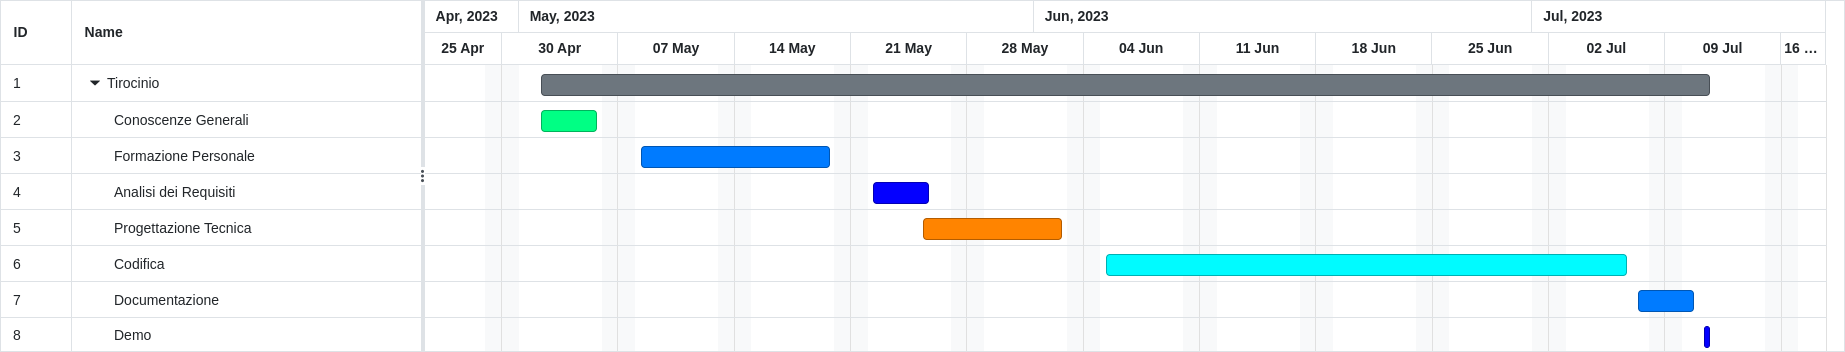
\includegraphics[width=350pt]{images/diagrammaGantt.png} 
    \caption{Diagramma di Gantt del tirocinio}
\end{figure}

    \chapter{Analisi dei requisiti}
\label{cap:analisi-requisiti}

\intro{Breve introduzione al capitolo}\\

\section{Casi d'uso}

Per lo studio dei casi di utilizzo del prodotto sono stati creati dei diagrammi.
I diagrammi dei casi d'uso (in inglese \emph{Use Case Diagram}) sono diagrammi di tipo \gls{uml} dedicati alla descrizione delle funzioni o servizi offerti da un sistema, così come sono percepiti e utilizzati dagli attori che interagiscono col sistema stesso.
Essendo il progetto finalizzato alla creazione di un tool per l'automazione di un processo, le interazioni da parte dell'utilizzatore devono essere ovviamente ridotte allo stretto necessario. Per questo motivo i diagrammi d'uso risultano semplici e in numero ridotto.

\begin{figure}[!h] 
    \centering 
    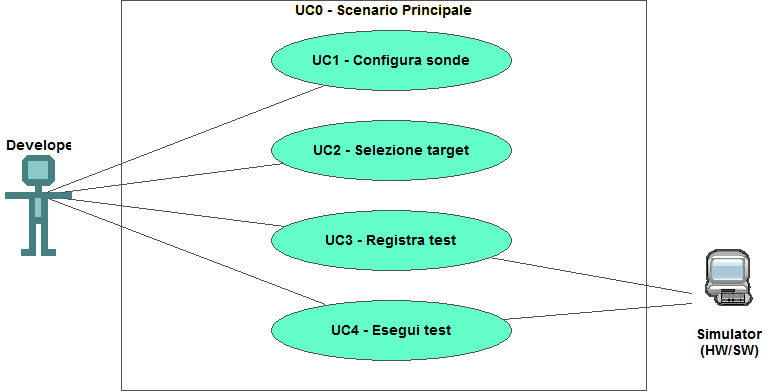
\includegraphics[width=0.9\columnwidth]{usecase/scenario-principale} 
    \caption{Use Case - UC0: Scenario principale}
\end{figure}

\begin{usecase}{0}{Scenario principale}
\usecaseactors{Sviluppatore applicativi}
\usecasepre{Lo sviluppatore è entrato nel plug-in di simulazione all'interno dell'IDE}
\usecasedesc{La finestra di simulazione mette a disposizione i comandi per configurare, registrare o eseguire un test}
\usecasepost{Il sistema è pronto per permettere una nuova interazione}
\label{uc:scenario-principale}
\end{usecase}

\section{Tracciamento dei requisiti}

Da un'attenta analisi dei requisiti e degli use case effettuata sul progetto è stata stilata la tabella che traccia i requisiti in rapporto agli use case.\\
Sono stati individuati diversi tipi di requisiti e si è quindi fatto utilizzo di un codice identificativo per distinguerli.\\
Il codice dei requisiti è così strutturato R(F/Q/V)(N/D/O) dove:
\begin{enumerate}
	\item[R =] requisito
    \item[F =] funzionale
    \item[Q =] qualitativo
    \item[V =] di vincolo
    \item[N =] obbligatorio (necessario)
    \item[D =] desiderabile
    \item[Z =] opzionale
\end{enumerate}
Nelle tabelle \ref{tab:requisiti-funzionali}, \ref{tab:requisiti-qualitativi} e \ref{tab:requisiti-vincolo} sono riassunti i requisiti e il loro tracciamento con gli use case delineati in fase di analisi.

\newpage

\begin{table}%
\caption{Tabella del tracciamento dei requisti funzionali}
\label{tab:requisiti-funzionali}
\begin{tabularx}{\textwidth}{lXl}
\hline\hline
\textbf{Requisito} & \textbf{Descrizione} & \textbf{Use Case}\\
\hline
RFN-1     & L'interfaccia permette di configurare il tipo di sonde del test & UC1 \\
\hline
\end{tabularx}
\end{table}%

\begin{table}%
\caption{Tabella del tracciamento dei requisiti qualitativi}
\label{tab:requisiti-qualitativi}
\begin{tabularx}{\textwidth}{lXl}
\hline\hline
\textbf{Requisito} & \textbf{Descrizione} & \textbf{Use Case}\\
\hline
RQD-1    & Le prestazioni del simulatore hardware deve garantire la giusta esecuzione dei test e non la generazione di falsi negativi & - \\
\hline
\end{tabularx}
\end{table}%

\begin{table}%
\caption{Tabella del tracciamento dei requisiti di vincolo}
\label{tab:requisiti-vincolo}
\begin{tabularx}{\textwidth}{lXl}
\hline\hline
\textbf{Requisito} & \textbf{Descrizione} & \textbf{Use Case}\\
\hline
RVO-1    & La libreria per l'esecuzione dei test automatici deve essere riutilizzabile & - \\
\hline
\end{tabularx}
\end{table}%


%\usepackage[dd/mm/yyyy]{datetime}
\hypersetup{
    bookmarks=false,    % show bookmarks bar?
    pdftitle={ENGaming-Analisi dei Requisiti},    % title
    pdfauthor={Nicola Baesso},                     % author
    pdfsubject={TeX and LaTeX},                        % subject of the document
    pdfkeywords={TeX, LaTeX, graphics, images}, % list of keywords
    colorlinks=true,       % false: boxed links; true: colored links
    linkcolor=blue,       % color of internal links
    citecolor=black,       % color of links to bibliography
    filecolor=black,        % color of file links
    urlcolor=purple,        % color of external links
    linktoc=page            % only page is linked
}

\chapter{Analisi dei requisiti}
\label{cap:analisi-requisiti}

\section{Casi d'uso}

In questo capitolo si illustrano i vari casi d'uso per il progetto ENGaming.\\
Per lo studio dei casi d'uso vengono utilizzati dei diagrammi, chiamati diagrammi dei casi d'uso (in inglese \emph{Use Case Diagram}).\\
Questi diagrammi sono diagrammi dei tipo \gls{uml}, dedicati alla descrizione delle funzioni offerte da un'applicativo, descrivendoli come sono percepiti e utilizzati dagli attori che interagiscono col sistema stesso.

\subsection{Attori}

Essendo questo prodotto rivolto agli utenti finali, l'unico attore presente nei casi d'uso è l'utente.\\
Non viene fatta una distinzione tra un utente generico ed un utente autenticato poichè non viene previsto che l'applicativo implementi un sistema di autenticazione.

\begin{figure}[h]
    \centering
    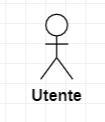
\includegraphics{images/usecase/attore.png}
    \caption{Attore presente nei casi d'uso}
    \label{fig:attore}
\end{figure}

\subsection{UC01 - Visualizzazione schermata iniziale}
\begin{figure}[h]
    \centering
    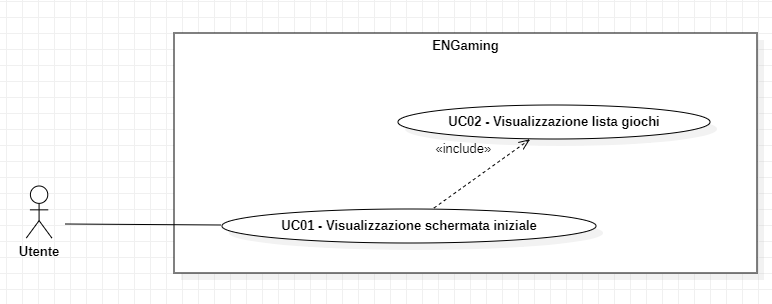
\includegraphics[width=400pt]{images/usecase/UC01.png}
    \caption{Diagramma per UC01}
    \label{fig:attore}
\end{figure}
\begin{itemize}
    \item Attore principale: Utente
    \item Pre-condizioni: l'utente non visualizza la schermata iniziale.
    \item Post-condizioni: l'utente visualizza la schermata iniziale.
    \item Scenario principale: \begin{itemize}
        \item Il sistema carica l'applicazione sul device ENSign11.
        \item L'utente arriva nella postazione in cui è presente il device.
        \item L'utente visualizza, sullo schermo del device, una lista di giochi selezionabile e un pulsante relativo ai record.
    \end{itemize}
    \item Include: \begin{itemize}
        \item UC02 - Visualizzazione lista giochi
    \end{itemize}
\end{itemize}

\subsection{UC02 - Visualizzazione lista giochi}
\begin{figure}[h]
    \centering
    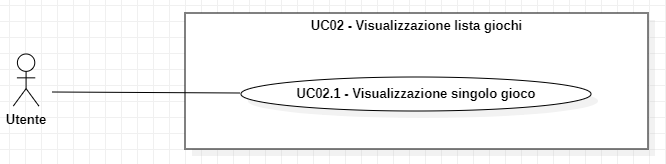
\includegraphics[width=400pt]{images/usecase/UC02.png}
    \caption{Diagramma per UC02}
    \label{fig:attore}
\end{figure}
\begin{itemize}
    \item Attore principale: Utente
    \item Pre-condizioni: l'utente non visualizza la lista dei giochi disponibili.
    \item Post-condizioni: l'utente visualizza la lista dei giochi disponibili.
    \item Scenario principale: \begin{itemize}
        \item L'utente visualizza una lista di giochi selezionabili. La lista è composta da icone che possono essere selezionate tramite il tocco. Essendo visualizzabili al massimo 10 icone, l'utente può effettuare uno scorrimento a sinistra o a destra per visualizzare le icone non visibili.
    \end{itemize}
    \item Include: \begin{itemize}
        \item UC02.1 - Visualizzazione singolo gioco
    \end{itemize}
\end{itemize}
\newpage
\subsection{UC02.1 - Visualizzazione singolo gioco}
\begin{figure}[h]
    \centering
    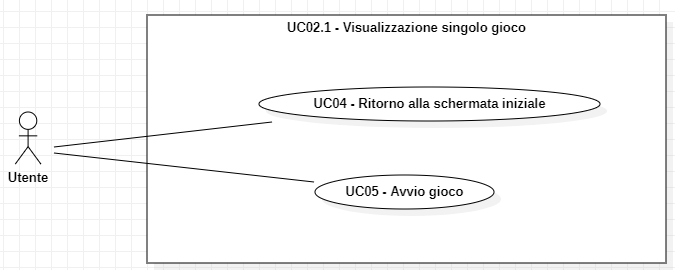
\includegraphics[width=400pt]{images/usecase/UC02_1.png}
    \caption{Diagramma per UC02.1}
    \label{fig:attore}
\end{figure}
\begin{itemize}
    \item Attore principale: Utente
    \item Pre-condizioni: l'utente sta visualizzando la lista dei giochi disponibili.
    \item Post-condizioni: l'utente visualizza le caratteristiche del singolo gioco.
    \item Scenario principale: \begin{itemize}
        \item L'utente, dalla lista di giochi selezionabili, seleziona un gioco.
        \item L'utente viene reindirizzato nella pagina del gioco scelto. Ogni gioco contiene, oltre all'apposito pulsante per iniziare a giocare, le seguenti informazioni: \begin{itemize}
            \item Nome del gioco
            \item Tipo di gioco (es. arcade, racing, action...)
            \item Descrizione del gioco, se presente
            \item Tipologia di input, tra controller e touch/digitalizer
            \item Mappatura dei comandi, se il gioco richiede l'uso del controller
        \end{itemize} Inoltre, la pagina contiene anche un pulsante per tornare alla schermata iniziale.
    \end{itemize}
    \item Include: \begin{itemize}
        \item UC04 - Ritorno alla schermata iniziale
        \item UC05 - Avvio gioco
    \end{itemize}
\end{itemize}
\newpage
\subsection{UC03 - Visualizzazione record}
\begin{figure}[h]
    \centering
    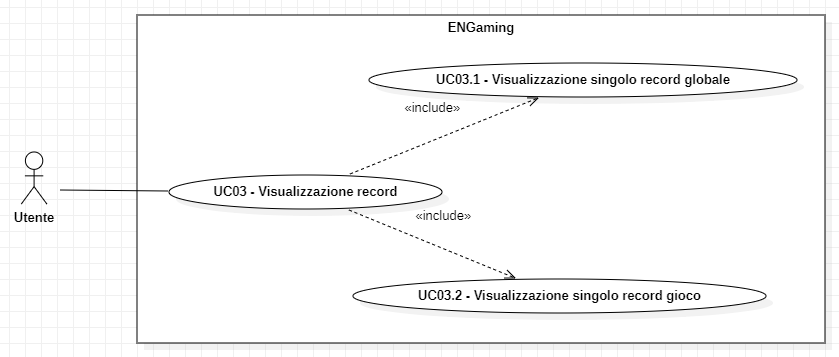
\includegraphics[width=400pt]{images/usecase/UC03.png}
    \caption{Diagramma per UC03}
    \label{fig:attore}
\end{figure}
\begin{itemize}
    \item Attore principale: Utente
    \item Pre-condizioni: l'utente si trova nella schermata principale, e non sta visualizzando i record.
    \item Post-condizioni: l'utente visualizza i record.
    \item Scenario principale: \begin{itemize}
        \item L'utente preme il pulsante relativo ai record, posto nell'area principale.
        \item L'utente, in una nuova pagina, visualizza la lista dei record globali, ovvero di tutti i record presenti nel device, ordinati per punteggio. In caso di punteggio uguale, i record vengono ordinati per data ed eventualmente per nome del gioco ascendente.
        \item L'utente, tramite un apposito bottone, rimane nella stessa pagina e può passare alle liste per gioco, visualizzando i record presenti per i singoli giochi, ordinati per punteggio. In caso di punteggio uguale, i record vengono ordinati per data.
    \end{itemize}
    \item Include: \begin{itemize}
        \item UC03.1 - Visualizzazione singolo record globale
        \item UC03.2 - Visualizzazione singolo record gioco
    \end{itemize}
\end{itemize}

\subsection{UC03.1 - Visualizzazione singolo record globale}
\begin{itemize}
    \item Attore principale: Utente
    \item Pre-condizioni: l'utente sta visualizzando la lista dei record globali.
    \item Post-condizioni: l'utente visualizza le caratteristiche del singolo record.
    \item Scenario principale: \begin{itemize}
        \item L'utente, dalla lista dei record presenti, ne vede i dettagli. Ogni record nella lista globale contiene le seguenti informazioni: \begin{itemize}
            \item Posizione in classifica
            \item Nome dell' utente che ha effettuato il record, composto da 3 lettere
            \item Punteggio conseguito
            \item Nome del gioco in cui si è fatto il record
        \end{itemize}
    \end{itemize}
\end{itemize}

\subsection{UC03.2 - Visualizzazione singolo record gioco}
\begin{itemize}
    \item Attore principale: Utente
    \item Pre-condizioni: l'utente sta visualizzando la lista dei record per un determinato gioco.
    \item Post-condizioni: l'utente visualizza le caratteristiche del singolo record.
    \item Scenario principale: \begin{itemize}
        \item L'utente, dalla lista dei record presenti, ne vede i dettagli. Ogni record nella lista di un determinato gioco contiene le seguenti informazioni: \begin{itemize}
            \item Posizione in classifica
            \item Nome dell' utente che ha effettuato il record, composto da 3 lettere
            \item Punteggio conseguito
        \end{itemize}
    \end{itemize}
\end{itemize}

\subsection{UC04 - Ritorno alla schermata iniziale}
\begin{itemize}
    \item Attore principale: Utente
    \item Pre-condizioni: l'utente vuole tornare alla schermata iniziale.
    \item Post-condizioni: l'utente si trova nella schermata iniziale.
    \item Scenario principale: \begin{itemize}
        \item L'utente preme l'apposito pulsante per ritornare nella schermata iniziale.
        \item Il sistema riceve l'input dal device e reindirizza l'utente verso la schermata iniziale.
    \end{itemize}
\end{itemize}

\newpage
\subsection{UC05 - Avvio gioco}
\begin{figure}[h]
    \centering
    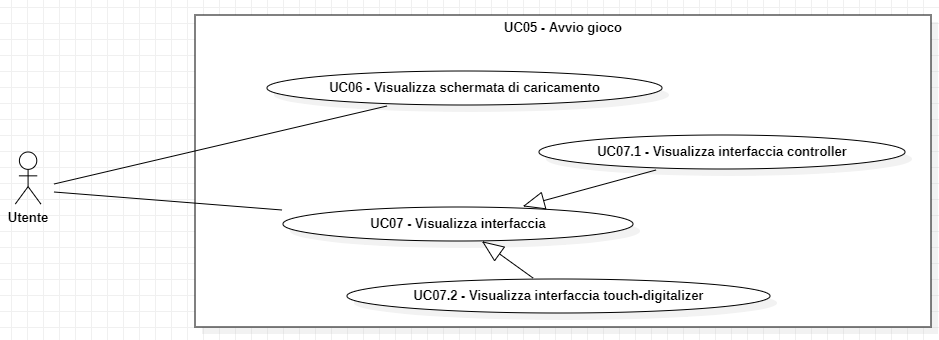
\includegraphics[width=400pt]{images/usecase/UC05.png}
    \caption{Diagramma per UC05}
    \label{fig:attore}
\end{figure}
\begin{itemize}
    \item Attore principale: Utente
    \item Pre-condizioni: l'utente sta visualizzando le caratteristiche del singolo gioco.
    \item Post-condizioni: l'utente è pronto per giocare.
    \item Scenario principale: \begin{itemize}
        \item L'utente, che si trova nella schermata di un gioco, avvia il gioco tramite l'apposito pulsante.
        \item L'utente visualizza una pagina di caricamento.
        \item Al termine del caricamento, l'utente visualizza una pagina con il gioco e l'interfaccia necessaria.
    \end{itemize}
    \item Include: \begin{itemize}
        \item UC06 - Visualizza schermata di caricamento
        \item UC07 - Visualizza interfaccia
    \end{itemize}
\end{itemize}

\subsection{UC06 - Visualizza schermata di caricamento}
\begin{itemize}
    \item Attore principale: Utente
    \item Pre-condizioni: l'utente ha iniziato l'avvio del gioco.
    \item Post-condizioni: il caricamento termina e l'utente è pronto per giocare.
    \item Scenario principale: \begin{itemize}
        \item L'utente, che si trova nella schermata di un gioco, avvia il gioco tramite l'apposito pulsante.
        \item L'utente visualizza una pagina di caricamento.\\ Questa pagina, completamente statica, mostra semplicemente una scritta che avvisa l'utente del caricamento, ad esempio "caricamento in corso".\\ La schermata deve rimanere su schermo per 4 secondi, indipendentemente dall'effettivo caricamento del gioco stesso.
    \end{itemize}
\end{itemize}

\subsection{UC07 - Visualizza interfaccia}
\begin{itemize}
    \item Attore principale: Utente
    \item Pre-condizioni: l'utente ha iniziato l'avvio del gioco ed ha appena superato la schermata di caricamento.
    \item Post-condizioni: il controller viene caricato e l'utente è pronto per giocare.
    \item Scenario principale: \begin{itemize}
        \item L'utente esce dalla schermata di caricamento.
        \item L'utente visualizza la pagina del gioco con l'interfaccia adatta al gioco stesso.
    \end{itemize}
\end{itemize}

\subsection{UC07.1 - Visualizza interfaccia controller}
\begin{itemize}
    \item Attore principale: Utente
    \item Pre-condizioni: l'utente ha iniziato l'avvio del gioco ed ha appena superato la schermata di caricamento.
    \item Post-condizioni: il controller viene caricato e l'utente è pronto per giocare.
    \item Scenario principale: \begin{itemize}
        \item L'utente esce dalla schermata di caricamento.
        \item L'utente visualizza la pagina del gioco con il controller.\\ Il controller è formato da quattro tasti direzionali, quattro tasti per le azioni ed un tasto di pausa.\\ Il posizionamento dei tasti deve permettere l'utilizzo del gioco senza prendere in mano il device utilizzato.
    \end{itemize}
\end{itemize}

\subsection{UC07.2 - Visualizza interfaccia touch-digitalizer}
\begin{itemize}
    \item Attore principale: Utente
    \item Pre-condizioni: l'utente ha iniziato l'avvio del gioco ed ha appena superato la schermata di caricamento.
    \item Post-condizioni: l'interfaccia viene caricata e l'utente è pronto per giocare.
    \item Scenario principale: \begin{itemize}
        \item L'utente esce dalla schermata di caricamento.
        \item L'utente visualizza la pagina del gioco con l'interfaccia per i comandi touch, o per l'utilizzo del digitalizer.\\ L'interfaccia è semplicemente formata dal tasto di pausa.\\ Il posizionamento del tasto deve permettere l'utilizzo del gioco senza occupare lo spazio necessario per lo stesso, od occupandone il meno possibile.
    \end{itemize}
\end{itemize}

\subsection{UC08 - Interazione gioco}
\begin{figure}[h]
    \centering
    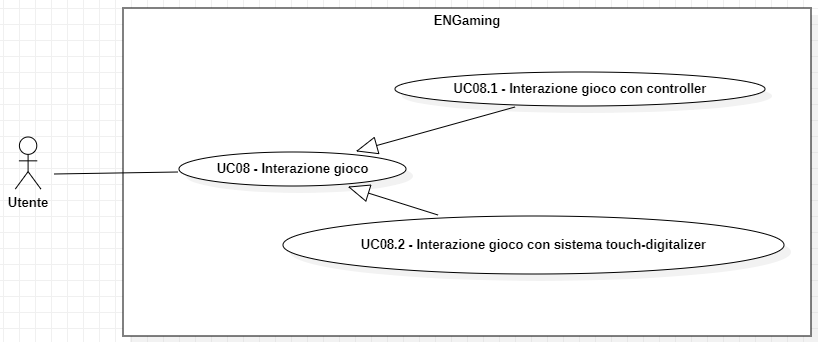
\includegraphics[width=400pt]{images/usecase/UC08.png}
    \caption{Diagramma per UC08}
    \label{fig:attore}
\end{figure}
\begin{itemize}
    \item Attore principale: Utente
    \item Pre-condizioni: l'utente vuole eseguire una determinata azione nel gioco.
    \item Post-condizioni: l'utente ha eseguito l'azione nel gioco.
    \item Scenario principale: \begin{itemize}
        \item L'utente esegue un azione attraverso l'interfaccia del gioco.
        \item Il sistema riceve l'input dell'interfaccia dal device e lo elabora.
        \item Il sistema prende il dato elaborato e lo manda al gioco.
    \end{itemize}
\end{itemize}

\subsection{UC08.1 - Interazione gioco con controller}
\begin{itemize}
    \item Attore principale: Utente
    \item Pre-condizioni: l'utente vuole eseguire una determinata azione nel gioco.
    \item Post-condizioni: l'utente ha eseguito l'azione nel gioco.
    \item Scenario principale: \begin{itemize}
        \item L'utente preme un pulsante nel controller.
        \item Il sistema riceve l'input del controller dal device e lo elabora.
        \item Il sistema prende il dato elaborato e lo manda al gioco.
    \end{itemize}
\end{itemize}

\subsection{UC08.2 - Interazione gioco con sistema touch-digitalizer}
\begin{itemize}
    \item Attore principale: Utente
    \item Pre-condizioni: l'utente vuole eseguire una determinata azione nel gioco.
    \item Post-condizioni: l'utente ha eseguito l'azione nel gioco.
    \item Scenario principale: \begin{itemize}
        \item L'utente esegue una gesture, ovvero un gesto, nel gioco.
        \item Il sistema riceve l'input del gesto dal device e lo elabora.
        \item Il sistema prende il dato elaborato e lo manda al gioco.
    \end{itemize}
\end{itemize}

\subsection{UC09 - Pausa del gioco}
\begin{figure}[h]
    \centering
    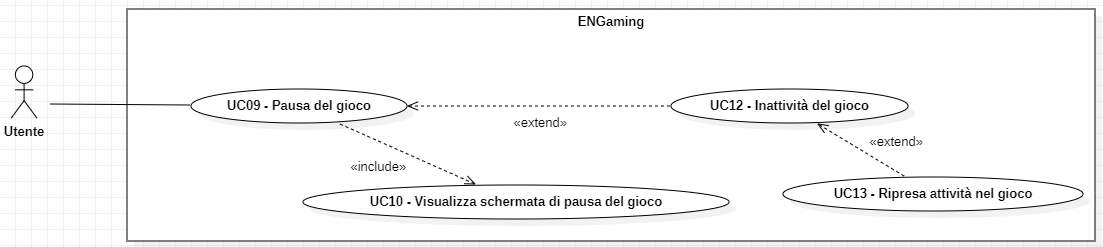
\includegraphics[width=400pt]{images/usecase/UC09.png}
    \caption{Diagramma per UC09}
    \label{fig:attore}
\end{figure}
\begin{itemize}
    \item Attore principale: Utente
    \item Pre-condizioni: l'utente vuole mettere in pausa il gioco.
    \item Post-condizioni: il gioco è in stato di pausa.
    \item Scenario principale: \begin{itemize}
        \item L'utente preme l'apposito pulsante di pausa.
        \item Il sistema riceve l'input dal device e mette in pausa il gioco.
        \item L'utente visualizza una pagina che informa dello stato di pausa del gioco.
    \end{itemize}
    \item Include: \begin{itemize}
        \item UC10 - Visualizza schermata di pausa del gioco
    \end{itemize}
    \item Estensioni: \begin{itemize}
        \item UC12 - Inattività del gioco
    \end{itemize}
\end{itemize}

\subsection{UC10 - Visualizza schermata di pausa del gioco}
\begin{figure}[h]
    \centering
    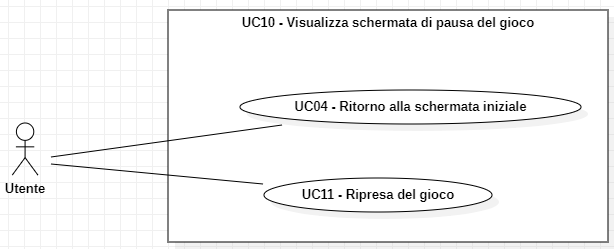
\includegraphics[width=400pt]{images/usecase/UC10.png}
    \caption{Diagramma per UC10}
    \label{fig:attore}
\end{figure}
\begin{itemize}
    \item Attore principale: Utente
    \item Pre-condizioni: L'utente ha messo in pausa il gioco.
    \item Post-condizioni: L'utente è informato dello stato di pausa del gioco.
    \item Scenario principale: \begin{itemize}
        \item L'utente visualizza una pagina che informa dello stato di pausa del gioco.\\ La pagina contiene una scritta che avvisa l'utente dello stato di pausa del gioco e due pulsanti.\\ Il primo pulsante permette di ricominciare a giocare, togliendo il gioco dallo stato di pausa, mentre il secondo permette di chiudere il gioco e tornare alla schermata iniziale.
    \end{itemize}
    \item Include: \begin{itemize}
        \item UC04 - Ritorno alla schermata iniziale
        \item UC11 - Ripresa del gioco
    \end{itemize}
\end{itemize}

\subsection{UC11 - Ripresa del gioco}
\begin{itemize}
    \item Attore principale: Utente
    \item Pre-condizioni: il gioco è in stato di pausa.
    \item Post-condizioni: il gioco è uscito dallo stato di pausa e l'utente può continuare a giocare.
    \item Scenario principale: \begin{itemize}
        \item L'utente preme l'apposito pulsante di ripresa del gioco.
        \item Il sistema riceve l'input dal device e toglie lo stato di pausa dal gioco.
    \end{itemize}
\end{itemize}

\subsection{UC12 - Inattività nel gioco}
\begin{itemize}
    \item Attore principale: Utente
    \item Pre-condizioni: l'utente non sta eseguendo alcuna attività sul gioco.
    \item Post-condizioni: il sistema visualizza la schermata iniziale.
    \item Scenario principale: \begin{itemize}
        \item Dopo 10 secondi dall'ultimo input, il sistema avvia un cronometro di 4 minuti.
        \item Al termine del cronometro, il sistema chiude il gioco e torna alla schermata iniziale.
    \end{itemize}
    \item Estensioni: \begin{itemize}
        \item UC13 - Ripresa attività nel gioco
    \end{itemize}
\end{itemize}

\subsection{UC13 - Ripresa attività nel gioco}
\begin{itemize}
    \item Attore principale: Utente
    \item Pre-condizioni: l'utente non sta eseguendo alcuna attività sul gioco.
    \item Post-condizioni: l'utente ha eseguendo un'attività sul gioco.
    \item Scenario principale: \begin{itemize}
        \item Dopo 10 secondi dall'ultimo input, il sistema avvia un cronometro di 4 minuti.
        \item L'utente esegue un'attività sul gioco prima dello scadere del cronometro.
        \item Il sistema interrompe il cronometro e lo riporta alla durata iniziale.
    \end{itemize}
\end{itemize}
\newpage
\subsection{UC14 - Inserimento nuovo record}
\begin{figure}[h]
    \centering
    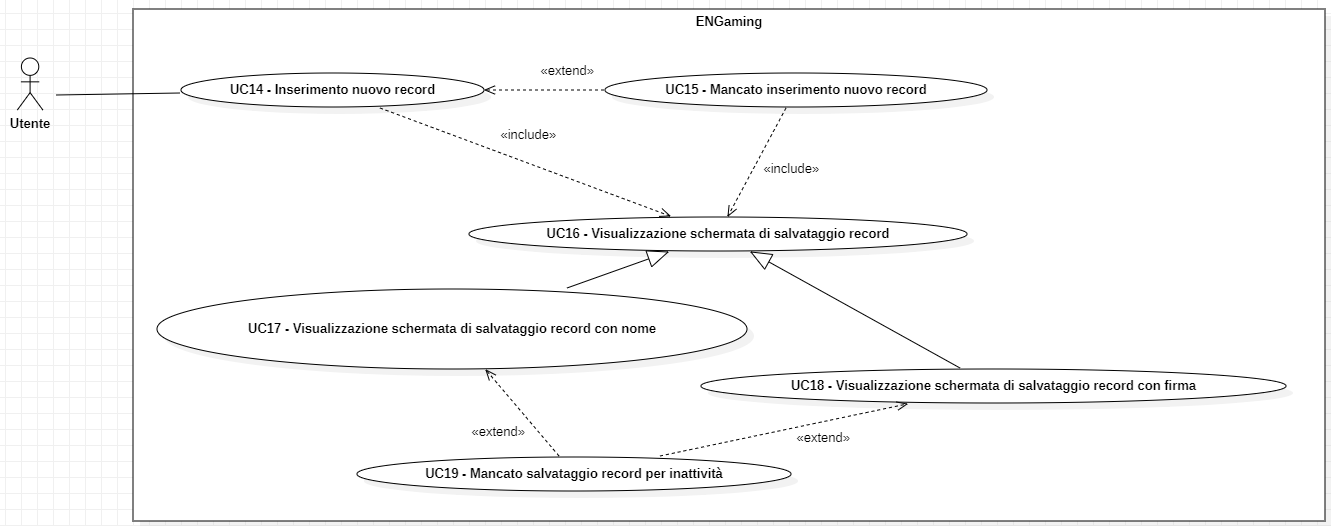
\includegraphics[width=410pt]{images/usecase/UC14.png}
    \caption{Diagramma per UC14}
    \label{fig:attore}
\end{figure}
\begin{itemize}
    \item Attore principale: Utente
    \item Pre-condizioni: l'utente chiude il gioco, ed ha effettuato un nuovo record.
    \item Post-condizioni: il sistema ha memorizzato il record effettuato dall'utente.
    \item Scenario principale: \begin{itemize}
        \item L'utente visualizza una schermata per informarlo della creazione di un nuovo record.
        \item Tramite la schermata, l'utente seleziona il metodo di salvataggio del record che più preferisce.
        \item Il sistema riceve il dato inserito dall'utente e memorizza il record.
    \end{itemize}
    \item Include: \begin{itemize}
        \item UC16 - Visualizzazione schermata di salvataggio record
    \end{itemize}
    \item Estensioni: \begin{itemize}
        \item UC15 - Mancato inserimento nuovo record 
    \end{itemize}
\end{itemize}

\subsection{UC15 - Mancato inserimento nuovo record}
\begin{itemize}
    \item Attore principale: Utente
    \item Pre-condizioni: l'utente ha effettuato un nuovo record in un gioco, ma non vuole salvarlo.
    \item Post-condizioni: il sistema non ha memorizzato il record effettuato dall'utente.
    \item Scenario principale: \begin{itemize}
        \item L'utente visualizza una schermata per informarlo della creazione di un nuovo record.
        \item Tramite la schermata, l'utente seleziona la volontà di non salvare il record effettuato.
        \item Il sistema scarta i dati relativi al record e non lo memorizza.
    \end{itemize}
    \item Include: \begin{itemize}
        \item UC16 - Visualizzazione schermata di salvataggio record
    \end{itemize}
\end{itemize}

\subsection{UC16 - Visualizzazione schermata di salvataggio record}
\begin{itemize}
    \item Attore principale: Utente
    \item Pre-condizioni: l'utente ha effettuato un nuovo record in un gioco.
    \item Post-condizioni: l'utente sta visualizzando la schermata relativa al salvataggio del record.
    \item Scenario principale: \begin{itemize}
        \item L'utente visualizza la schermata che lo informa della creazione di un nuovo record, e ne propone il salvataggio.\\ Questa schermata, oltre a riportare il punteggio del record, propone tre opzioni: il salvataggio del record tramite nome, il salvataggio del record tramite firma e il non salvataggio del record.
    \end{itemize}
\end{itemize}

\subsection{UC17 - Visualizzazione schermata di salvataggio record con nome}
\begin{itemize}
    \item Attore principale: Utente
    \item Pre-condizioni: l'utente vuole salvare il record con il proprio nome.
    \item Post-condizioni: l'utente ha inserito il proprio nome correttamente.
    \item Scenario principale: \begin{itemize}
        \item L'utente visualizza la schermata di salvataggio tramite nome.\\ Il nome può essere inserito tramite due pulsanti per carattere, ognuno dei quali passa al carattere precedente o al successivo.\\ Una volta che l'utente è soddisfatto, può premere l'apposito pulsante per il salvataggio del nome.
    \end{itemize}
    \item Estensioni: \begin{itemize}
        \item UC19 - Mancato salvataggio record per inattività
    \end{itemize}
\end{itemize}


\subsection{UC18 - Visualizzazione schermata di salvataggio record con firma}
\begin{itemize}
    \item Attore principale: Utente
    \item Pre-condizioni: l'utente vuole salvare il record con la propria firma.
    \item Post-condizioni: l'utente ha inserito la propria firma correttamente.
    \item Scenario principale: \begin{itemize}
        \item L'utente visualizza la schermata di salvataggio tramite firma.\\ La firma può essere inserita sia tramite l'utilizzo del touch screen, quindi firmando con il dito, sia tramite l'utilizzo del digitalizer.\\ Una volta che l'utente è soddisfatto, può premere l'apposito pulsante per il salvataggio della firma.
    \end{itemize}
    \item Estensioni: \begin{itemize}
        \item UC19 - Mancato salvataggio record per inattività
    \end{itemize}
\end{itemize}

\subsection{UC19 - Mancato salvataggio record per inattività}
\begin{itemize}
    \item Attore principale: Utente
    \item Pre-condizioni: l'utente non sta eseguendo alcuna attività \\ sulla schermata di salvataggio record.
    \item Post-condizioni: il record non viene salvato nel sistema.
    \item Scenario principale: \begin{itemize}
        \item Dopo 10 secondi dall'ultima interazione, il sistema avvia un cronometro di 4 minuti.
        \item Al termine del cronometro, il sistema chiude la schermata di salvataggio record, non salva il record e torna alla schermata iniziale.
    \end{itemize}
\end{itemize}
\newpage
\section{Requisiti}
In questa sezione vengono elencati i requisiti analizzati per l'applicativo.\\
Le tabelle, suddivide per tipologia di requisito, forniscono le seguenti informazioni:
\begin{itemize}
    \item \textbf{Codice}, che indica la tipologia di requisito (tra F=funzionale, Q=qualità e V=vincolo) e il numero del requisito.
    \item \textbf{Requisito}, dove si indica il requisito vero e proprio.
    \item \textbf{Tipologia}, ovvero se il requisito indicato è obbligatorio oppure opzionale.
    \item \textbf{Caso d'uso} di riferimento (solo per i requisiti funzionali).
\end{itemize}
\subsection{Requisiti funzionali}
\begin{longtable}{|c|c|c|c|}
    \hline
    \thead{Codice}&\thead{Requisito}&\thead{Tipologia}&\thead{Caso d'uso}\\
    \hline
    RF01&\makecell{Dev'essere possibile \\ visualizzare la lista \\ di giochi disponibili}&Obbligatorio&UC01,UC02\\
    \hline
    RF02&\makecell{Dev'essere possibile \\ effettuare uno scorrimento per \\ visualizzare le icone nascoste}&Obbligatorio&UC02\\
    \hline
    RF03&\makecell{Dev'essere possibile \\ toccare le icone presenti nella \\ schermata iniziale}&Obbligatorio&UC01,UC02,UC03\\
    \hline
    RF04&\makecell{Dev'essere possibile \\ visualizzare le informazioni \\ relative ad un singolo gioco}&Obbligatorio&UC02.1\\
    \hline
    RF05&\makecell{Dev'essere possibile \\ visualizzare la lista \\ dei record globale}&Obbligatorio&UC03\\
    \hline
    RF06&\makecell{Dev'essere possibile \\ visualizzare la lista \\ dei record per ogni gioco presente}&Obbligatorio&UC03\\
    \hline
    RF07&\makecell{Dev'essere possibile \\ effettuare uno scorrimento \\ per visualizzare i record nascosti}&Obbligatorio&UC03\\
    \hline
    RF08&\makecell{Dev'essere possibile \\ visualizzare le informazioni \\ relative ad un singolo record}&Obbligatorio&UC03.1,UC03.2\\
    \hline
    RF09&\makecell{Dev'essere possibile \\ ritornare alla schermata iniziale}&Obbligatorio&UC04\\
    \hline
    RF10&\makecell{Dev'essere possibile \\ avviare un gioco}&Obbligatorio&UC05\\
    \hline
    RF11&\makecell{Dev'essere possibile \\ visualizzare una pagina \\ di caricamento}&Obbligatorio&UC06\\
    \hline
    RF12&\makecell{La pagina di caricamento \\ dev'essere visibile \\ per almeno 4 secondi}&Obbligatorio&UC06\\
    \hline
    RF13&\makecell{Dev'essere possibile \\ l'utilizzo di \\ un controller virtuale}&Obbligatorio&UC07.1\\
    \hline
    RF14&\makecell{Il controller \\ deve avere nove tasti}&Obbligatorio&UC07.1\\
    \hline
    RF15&\makecell{Il controller \\ non deve richiede \\ l'impugnatura del device utilizzato}&Obbligatorio&UC07.1\\
    \hline
    RF16&\makecell{Dev'essere possibile \\ giocare utilizzando le dita delle mani}&Obbligatorio&UC07.2\\
    \hline
    RF17&\makecell{Dev'essere possibile \\ giocare utilizzando il digitalizer}&Obbligatorio&UC07.2\\
    \hline
    RF18&\makecell{Il pulsante di pausa \\ deve occupare il meno possibile \\ l'area di gioco}&Obbligatorio&UC07.2\\
    \hline
    RF19&\makecell{Dev'essere possibile \\ interagire con un gioco \\ attraverso il controller}&Obbligatorio&UC08.1\\
    \hline
    RF20&\makecell{Dev'essere possibile \\ interagire con un gioco \\ attraverso le dita delle mani}&Obbligatorio&UC8.2\\
    \hline
    RF21&\makecell{Dev'essere possibile \\ interagire con un gioco \\ attraverso il digitalizer}&Obbligatorio&UC8.2\\
    \hline
    RF22&\makecell{Dev'essere possibile \\ mettere in pausa \\ un gioco}&Obbligatorio&UC09\\
    \hline
    RF23&\makecell{Il sistema deve avvisare \\ quando un gioco \\ è in pausa}&Obbligatorio&UC09,UC10\\
    \hline
    RF24&\makecell{Dev'essere possibile \\ far ripartire un gioco \\ dopo la pausa}&Obbligatorio&UC10,11\\
    \hline
    RF25&\makecell{Dev'essere possibile \\ chiudere un gioco e tornare \\ alla schermata iniziale}&Obbligatorio&UC10,UC04\\
    \hline
    RF26&\makecell{Il sistema deve tornare \\ alla schermata iniziale \\ dopo 4 minuti di inattività}&Obbligatorio&UC12,UC19\\
    \hline
    RF27&\makecell{Il sistema deve far partire \\ il cronometro di inattività \\ dopo 10 secondi dall'ultimo input}&Obbligatorio&UC12,UC19\\
    \hline
    RF28&\makecell{Il sistema deve interrompere \\ il cronometro di inattività all'azione \\ dell'utente, prima del suo scadere}&Obbligatorio&UC13\\
    \hline
    RF29&\makecell{Dev'essere possibile \\ memorizzare un nuovo record}&Obbligatorio&UC14\\
    \hline
    RF30&\makecell{L'utente deve poter scegliere \\ se salvare o no \\ il record effettuato}&Obbligatorio&UC14,UC15,UC16\\
    \hline
    RF31&\makecell{L'utente deve visualizzare \\ la schermata dove decidere \\ se salvare un record}&Obbligatorio&UC16\\
    \hline
    RF32&\makecell{L'utente deve poter salvare \\ il record \\ tramite il suo nome}&Obbligatorio&UC17\\
    \hline
    RF33&\makecell{L'utente deve poter \\ inserire il suo nome}&Obbligatorio&UC17\\
    \hline
    RF34&\makecell{L'utente deve poter salvare \\ il record \\ tramite la sua firma}&Opzionale&UC18\\
    \hline
    RF35&\makecell{L'utente deve poter \\ inserire la sua firma}&Opzionale&UC18\\
    \hline
    RF36&\makecell{Il sistema non deve \\ salvare il record \\ in caso di inattività}&Obbligatorio&UC19\\
    \hline
\end{longtable}
\subsection{Requisiti di qualità}
    \begin{longtable}{|c|c|c|c|} 
        \hline
        \thead{Codice}&\thead{Requisito}&\thead{Tipologia}\\
        \hline
        RQ01 &\makecell{Dev'essere fornita la documentazione necessaria \\ per l'utilizzo del prodotto} & Obbligatorio\\
        \hline
        RQ02 & \makecell{Dev'essere fornita la documentazione necessaria \\ per la manuntenzione del prodotto} & Obbligatorio\\ 
        \hline
        RQ03 & \makecell{Il prodotto dev'essere versionato e pubblicato \\ sulle piattaforme aziendali} & Obbligatorio\\
        \hline
    \end{longtable}
\subsection{Requisiti di vincolo}
\begin{longtable}{|c|c|c|c|}
    \hline
    \thead{Codice}&\thead{Requisito}&\thead{Tipologia}\\
    \hline
    RV01 & \makecell{L'interfaccia grafica del prodotto \\ dev'essere sviluppata utilizzando \\ i linguaggi HTML, CSS, Javascript e Typescript} & Obbligatorio\\
    \hline
    RV02 & \makecell{L'interfaccia grafica del prodotto \\ dev'essere sviluppata utilizzando \\ il framework Angular} & Obbligatorio\\
    \hline
    RV03 & \makecell{L'interfaccia grafica del prodotto \\ dev'essere sviluppata utilizzando \\ il framework Electron} & Obbligatorio\\
    \hline
    RV04 & \makecell{Il prodotto dev'essere utilizzabile \\ attraverso il device ENSign 11} & Obbligatorio\\
    \hline
    RV05 & \makecell{Il prodotto deve utilizzare \\ il linguaggio C++ per la ricezione dei dati dal device} & Obbligatorio\\
    \hline
    RV06 & \makecell{Il prodotto dev'essere utilizzabile \\ senza impugnare il device} & Obbligatorio\\
    \hline
    RV07 & \makecell{Il prodotto dev'essere utilizzabile \\ attraverso il sistema touch screen del device} & Obbligatorio\\
    \hline
    RV08 & \makecell{Il prodotto dev'essere utilizzabile \\ attraverso il digitalizer presente nel device} & Obbligatorio\\
    \hline
\end{longtable}

    \chapter{Progettazione e codifica}
\label{cap:progettazione-codifica}

\section{Tecnologie e strumenti}
\label{sec:tecnologie-strumenti}

In questa sezione, si descrivono le tecnologie utilizzate sia per ENGaming sia per i giochi.\\
Infatti, nonostante i giochi non necessitino di modifiche per il funzionamento in ENGaming, ritengo comunque opportuno citarne le tecnologie che utilizzano, che ritengo possano essere interessanti.

\subsection{Tecnologie e strumenti del prodotto}

\subsubsection{Electron}
\begin{figure}[h]
    \centering
    
\includegraphics[width=150pt]{images/technologies/electron.png}
    \caption{Logo di Electron}
    \label{fig:electron}
\end{figure}
\gls{elctr} viene utilizzato per creare l'applicazione desktop, visualizzandola nello schermo dell'ENSign11.\\
Inoltre, si occupa della comunicazione tra il back-end e il front-end dell'applicazione, attraverso canali \gls{ipcg}.

\subsubsection{Angular}
\begin{figure}[h]
    \centering
    
\includegraphics[width=150pt]{images/technologies/angular.png}
    \caption{Logo di Angular}
    \label{fig:angular}
\end{figure}
\gls{angl} è il framework scelto per la realizzazione della parte visiva dell'applicazione.\\
\emph{Angular} permette la creazione di Componenti, ovvero di elementi o pagine, dove sono presenti:
\begin{itemize}
    \item un file HTML, per la visualizzazione del componente.
    \item un foglio di stile (CSS/SASS/LESS) per gli effetti grafici.
    \item un file Typescript, per definire il comportamento del componente.
\end{itemize}
Inoltre, permette l'utilizzo di Servizi per il trasferimento di dati tra componenti.
\subsubsection{Typescript}
\begin{figure}[h]
    \centering
    
\includegraphics[width=150pt]{images/technologies/typescript.png}
    \caption{Logo di Typescript}
    \label{fig:typescript}
\end{figure}
\gls{tsc} viene utilizzato sia da Electron che da Angular (da quest'ultimo per la definizione del comportamento di componenti e servizi).\\
Ciò che caratterizza Typescript da Javascript è la tipizzazione delle variabili, elemento che trovo molto utile sopratutto se si è in precedenza lavorato con linguaggi di programmazione come Java e C++, come nel mio caso.\\
I sorgenti scritti in questo linguaggio devono poi essere compilati per generare il file Javascript effettivamente letto dal browser.

\subsubsection{C++}
\begin{figure}[h]
    \centering
    
\includegraphics[width=150pt]{images/technologies/cpp.png}
    \caption{Logo di C++}
    \label{fig:cpp}
\end{figure}
\gls{cpp} è utilizzato per la logica relativa al device. In particolare, attraverso un driver (fornito dall'azienda), si possono rilevare le interazioni con il device (sia tramite tocco che tramite digitalizer).

\subsubsection{Node-API}
\begin{figure}[h]
    \centering
    
\includegraphics[width=150pt]{images/technologies/nodeapi.png}
    \caption{Logo delle Node-API}
    \label{fig:nodeapi}
\end{figure}
Le \gls{napi} sono utilizzate per rendere la parte in C++ "usabile" dalla parte sviluppata in Electron.\\
Infatti, senza di esse, non sarebbe possibile utilizzare i metodi per l'interazione con il device.

\subsubsection{Electron-Forge}
\gls{elctrForge} viene utilizzato per creare degli installer, o dei pacchetti, a seconda del sistema operativo in cui si va a compilare il progetto.\\
Tale strumento permette di compilare l'applicazione per Windows, Linux e MacOS, e ciò rende ENGaming un applicativo multipiattaforma.

\subsection{Tecnologie e strumenti dei giochi}

\subsubsection{HTML-CSS-JavaScript}
\begin{figure}[h]
    \centering
    
\includegraphics[width=300pt]{images/technologies/HTMLCSSJS.png}
    \caption{Loghi di HTML, CSS e Javascript}
    \label{fig:HTMLCSSJS}
\end{figure}
I giochi che ENGaming esegue sono semplici giochi eseguibili anche su browser. Per tale motivo, sono scritti con HTML per la struttura (generalmente composta da canvas), CSS per lo stile e Javascript per il gioco vero e proprio.\\
Per avere tutte le funzionalità che l'applicativo offre, è necessario che i giochi implementino una piccola modifica (spiegata più avanti).

\subsubsection{WebAssembly}
\begin{figure}[h]
    \centering
    
\includegraphics[width=150pt]{images/technologies/webassembly.png}
    \caption{Logo di WebAssembly}
    \label{fig:webassembly}
\end{figure}
Nel caso si volesse eseguire un classico nell'ENGaming (ad esempio, Doom), bisogna prima passare per \gls{webassembly}, in modo da renderlo eseguibile su un browser.

\section{Progettazione}
\label{sec:progettazione}
\subsection{Classi utilizzate}
\begin{figure}[h]
    \centering
    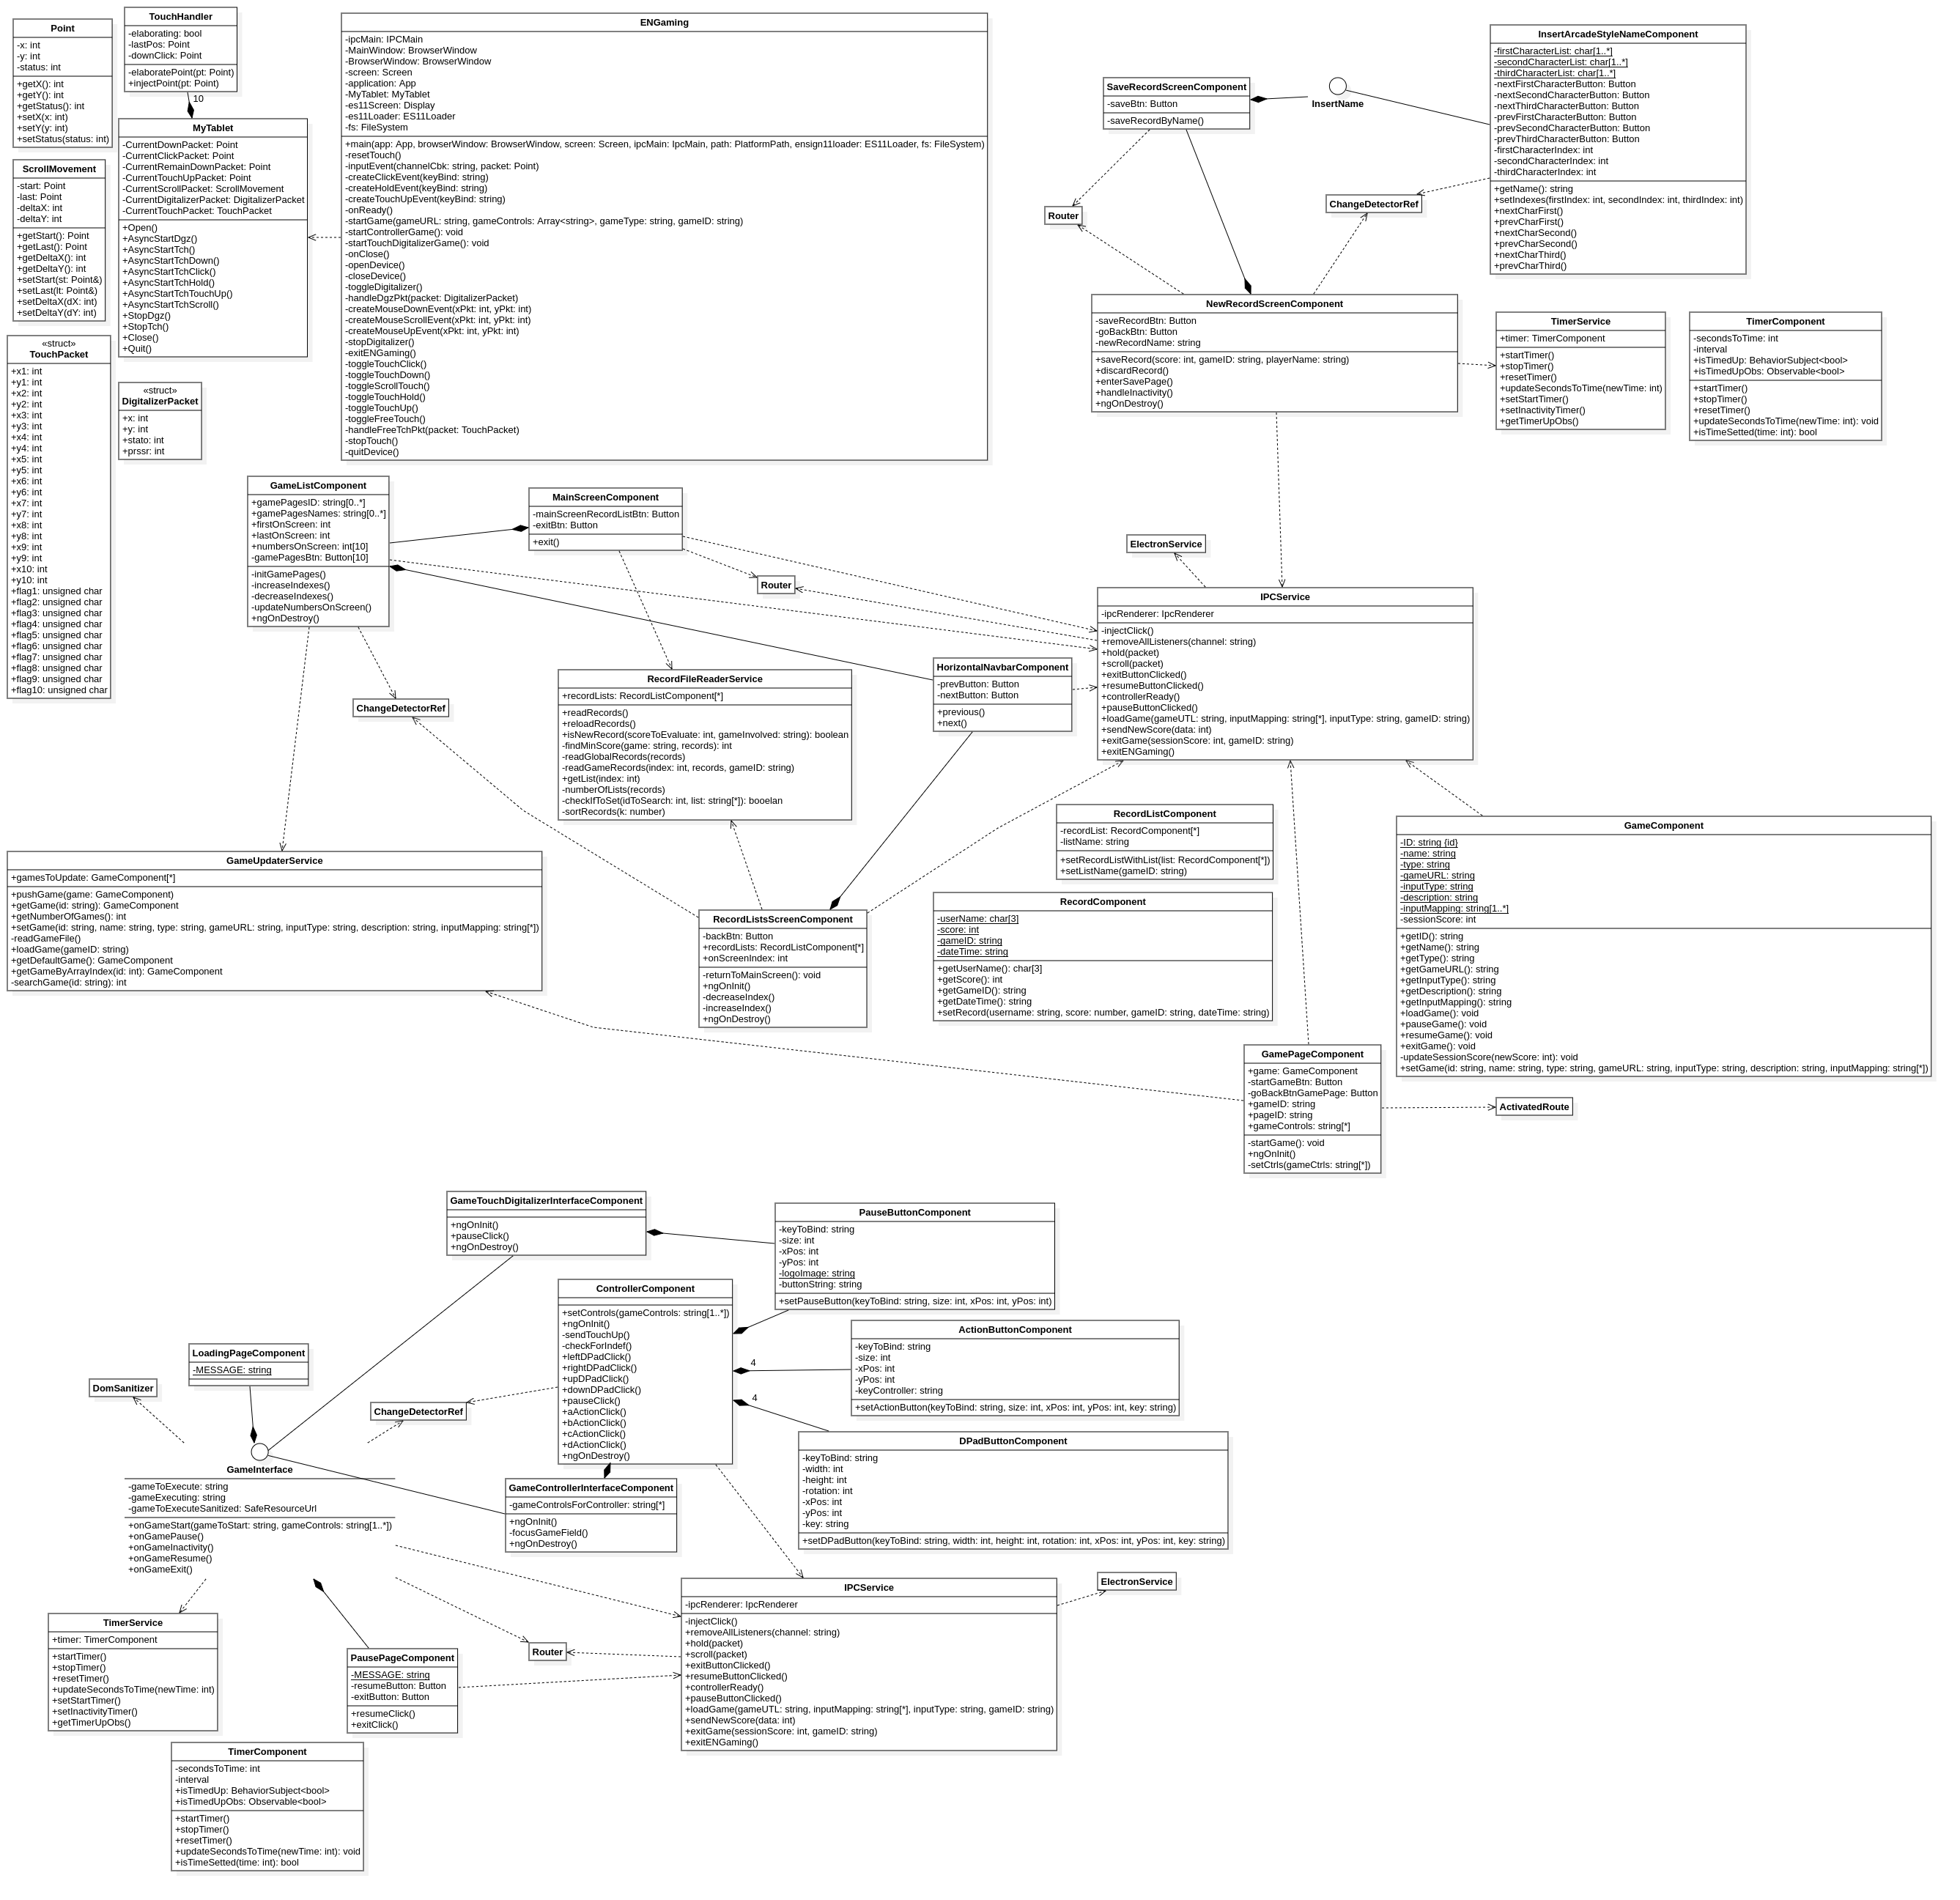
\includegraphics[width=340pt]{images/prog/ENGaming.png}
    \caption{Diagramma completo delle classi utilizzate}
    \label{fig:diagrammaCompleto}
\end{figure}
% immagine grafico completo
Le classi utilizzate possono essere classificate tramite il linguaggio d'implementazione:
\begin{itemize}
    \item Electron: \begin{itemize}
        \item ENGaming
    \end{itemize}
    \item C++: \begin{itemize}
        \item MyTablet
        \item TouchHandler
        \item Point
        \item ScrollMovement
        \item TouchPacket
        \item DigitalizerPacket
    \end{itemize}
    \item Angular: \begin{itemize}
        \item Tutte le classi "Component"
        \item Tutte le classi "Service"
        \item GameInterface
        \item InsertName
        \item Router
        \item ChangeDetectorRef
        \item DomSanitizer
        \item ActivatedRoute
    \end{itemize}
\end{itemize}
Di seguito si analizzano le vari componenti con maggior dettaglio.
\newpage
\subsubsection{ENGaming}
\begin{figure}[h]
    \centering
    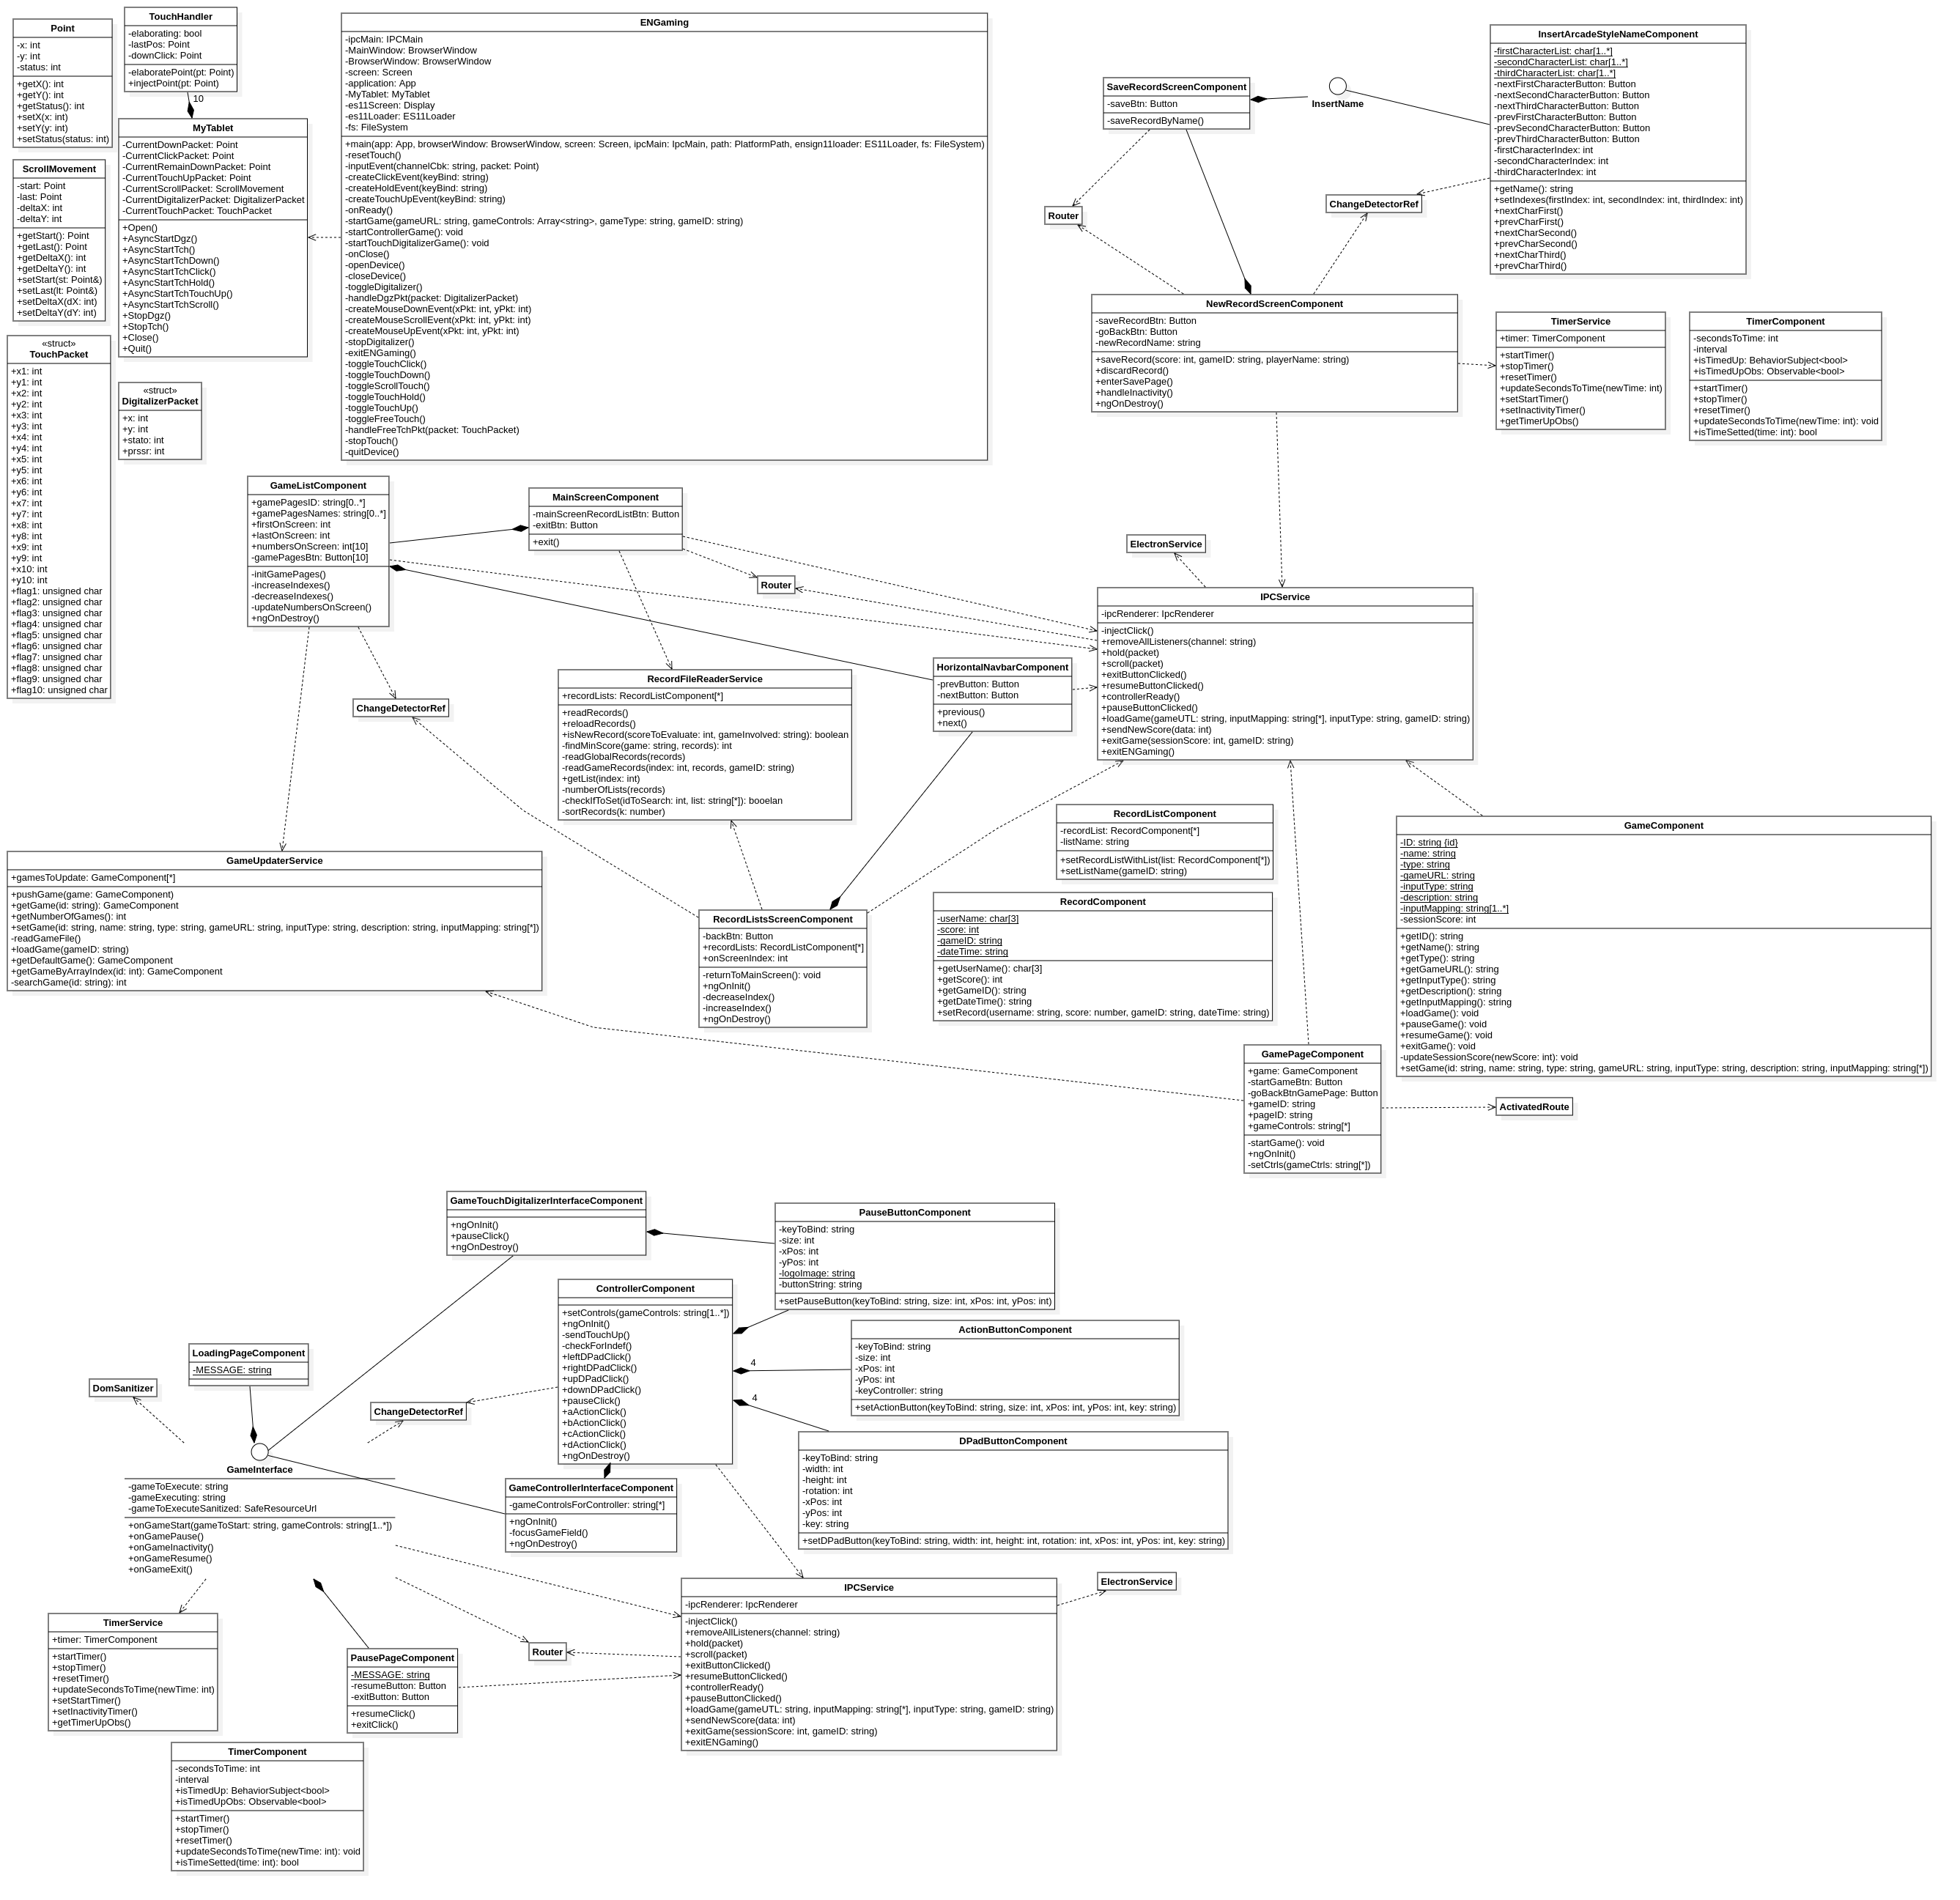
\includegraphics[width=340pt]{images/prog/ENGaming.png}
    \caption{Classe ENGaming}
    \label{fig:engaming}
\end{figure}
% immagine dettaglio ENGaming
La classe \emph{ENGaming} si occupa dell'avvio dell'applicazione.\\ Sviluppata in \gls{elctr}, contiene i componenti necessari per la creazione della finestra nell'ENSign 11 (Screen, BrowserWindow) e per la comunicazione con la parte in \gls{angl} (IPCMain).\\
Inoltre, contiene anche i moduli per la comunicazione con ENSign11.\\
Contiene:
\begin{itemize}
    \item i metodi per interagire con l'ENSign11: \begin{itemize}
        \item \emph{openDevice}, per aprire il device.
        \item \emph{toggleTouchClick}, per ricevere un click.
        \item \emph{toggleTouchDown}, per ricevere un down, ovvero l'evento di un dito appoggiato sullo schermo del device.
        \item \emph{toggleTouchHold}, per ricevere un hold, ovvero l'evento di un dito ancora appoggiato sullo schermo del device.
        \item \emph{toggleTouchUp}, per ricevere un touch up, ovvero l'evento di un dito sollevato dallo schermo del device.
        \item \emph{toggleScrollTouch}, per ricevere un evento di scroll, ovvero un evento di movimento di un dito sullo schermo del device.
        \item \emph{toggleFreeTouch}, per ricevere i pacchetti definiti nella struttura \emph{TouchPacket}.
        \item \emph{stopTouch}, per fermare le interazioni con lo schermo del device.
        \item \emph{toggleDigitalizer}, per ricevere i pacchetti definiti nella struttura \emph{DigitalizerPacket}.
        \item \emph{stopDigitalizer}, per fermare le interazioni con il digitalizer.
        \item \emph{closeDevice}, per chiudere il device.
        \item \emph{quitDevice}, per "liberare" il device e renderlo disponibile ad altri applicativi (o a una nuova istanza di ENGaming).
    \end{itemize}
    \item i metodi per l'avvio dei giochi: \begin{itemize}
        \item \emph{startGame}: identifica la tipologia del gioco e lo inizializza.
        \item \emph{startControllerGame}: inizializza un gioco che richiede l'uso del controller.
        \item \emph{startTouchDigitalizerGame}: inizializza un gioco che richiede l'uso del dito o del digitalizer.
    \end{itemize}
    \item i metodi per interagire con un gioco che utilizza il controller: \begin{itemize}
        \item \emph{inputEvent}, che permette l'interazione con il controller, nell'apposito componente.
        \item \emph{createClickEvent}, che crea l'evento "click" nella pagina del gioco.
        \item \emph{createHoldEvent}, che crea l'evento "hold" nella pagina del gioco.
        \item \emph{createTouchUpEvent}, che crea l'evento "touch up" nella pagina del gioco.
    \end{itemize}
    \item i metodi per interagire con un gioco che utilizza il dito o il digitalizer: \begin{itemize}
        \item \emph{handleFreeTchPkt}: in base allo stato del pacchetto, si decide che evento sollevare.
        \item \emph{handleDgzPkt}: come per \emph{handleFreeTchPkt}, per il digitalizer.
        \item \emph{createMouseDownEvent}: crea l'evento di appoggio del dito/digitalizer nel gioco.
        \item \emph{createMouseScrollEvent}, crea l'evento di movimento del dito/digitalizer nel gioco.
        \item \emph{createMouseUpEvent}, crea l'evento di sollevamento del dito/digitalizer nel gioco.
    \end{itemize}
    \item \emph{resetTouch}: ripristina il touch del device alla fine di un gioco.
    \item \emph{exitENGaming}: chiude l'applicazione.
\end{itemize}
\newpage
\subsubsection{Schermata iniziale}
\begin{figure}[h]
    \centering
    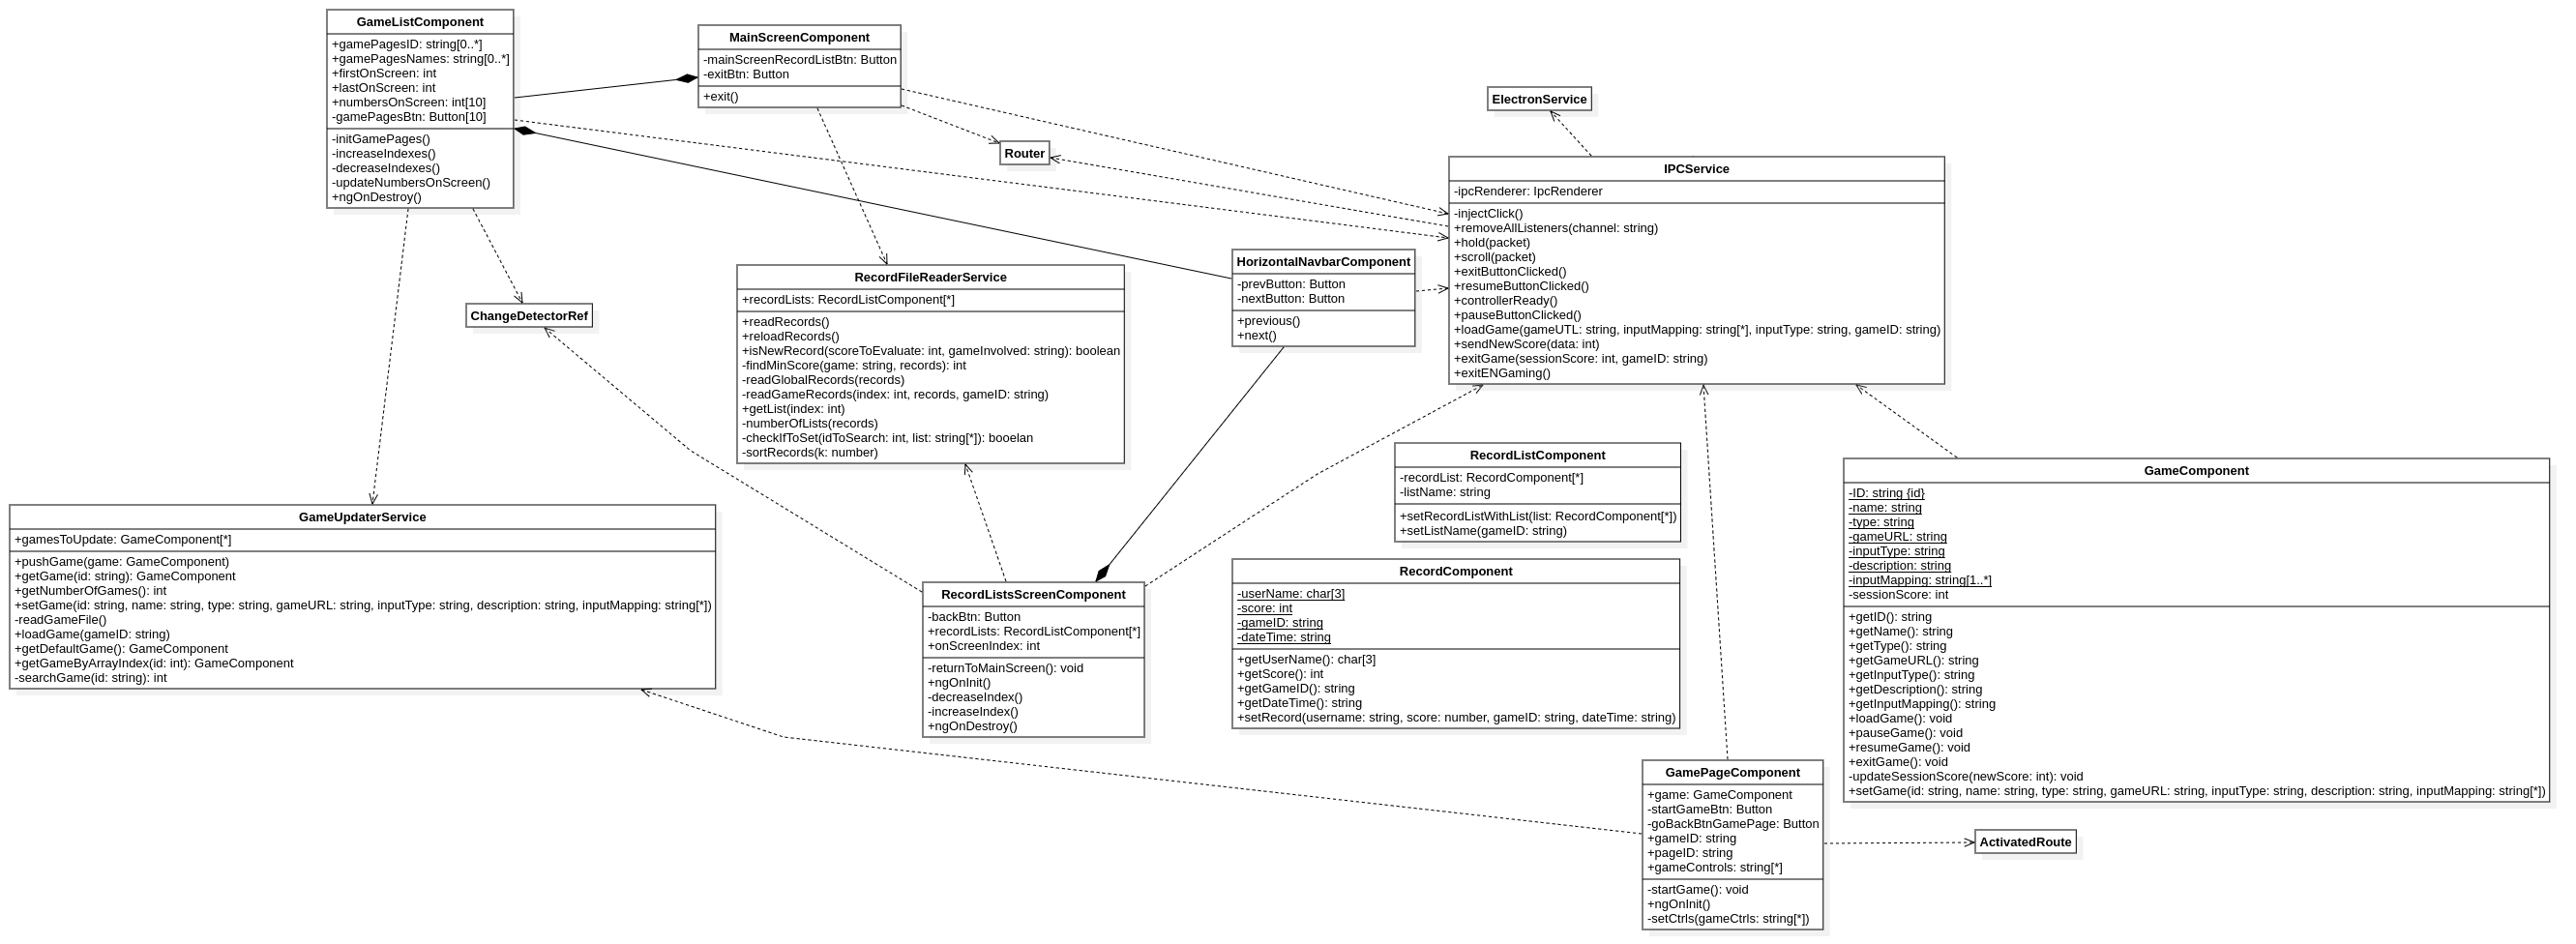
\includegraphics[width=340pt]{images/prog/MainScreen.png}
    \caption{Classi della schermata iniziale}
    \label{fig:schermataIniziale}
\end{figure}
% immagine dettaglio schermata iniziale
All'avvio dell'applicazione, la schermata iniziale presenta tre elementi:
\begin{itemize}
    \item L'elenco dei giochi disponibili, ottenuto da \emph{GameListComponent}.
    \item Il pulsante per accedere alla pagina di \emph{RecordListScreenComponent}.
    \item Il pulsante per uscire dall'applicazione.
\end{itemize}
Inoltre, il componente che gestisce questa schermata, ovvero \emph{MainScreenComponent}, si serve del service \emph{IPCService} per le comunicazioni attraverso le altre componenti dell'applicazione, utilizzando i canali IPC.
A sua volta:
\begin{itemize}
    \item \emph{RecordListScreenComponent} è formato da almeno un \emph{RecordListComponent}, poichè la schermata ha almeno la lista globale dei record. Inoltre, utilizza il \emph{HorizontalNavbarComponent} per navigare tra una lista e l'altra.
    \item \emph{RecordListComponent} contiene il nome della lista stessa e utilizza \emph{IPCService} per la comunicazione con il resto dell'applicazione.\\ Ovviamente, contiene anche vari \emph{RecordComponent}.
    \item \emph{GameListComponent} è formato sia dall' \emph{HorizontalNavbarComponent},\\ poichè gestisce la visualizzazione della lista di giochi disponibili, sia da almeno una \emph{GamePageComponent}, ossia da almeno una pagina relativa a un gioco.
    \item Ogni \emph{GamePageComponent} è relativa a un solo \emph{GameComponent}, le cui informazioni sono caricate da GameUpdaterService. Contiene sia il \emph{GameComponent}, sia i pulsanti per avviare il gioco e per tornare alla schermata principale.
\end{itemize}
\emph{GameComponent} e \emph{RecordComponent} utilizzano anche determinate proprietà, che si elencano negli appositi paragrafi rispettivamente in \nameref{subsec:gameComponent} e \nameref{subsec:recordComponent}.
\newpage
\subsubsection{GameComponent}
\label{subsec:gameComponent}
\begin{figure}[h]
    \centering
    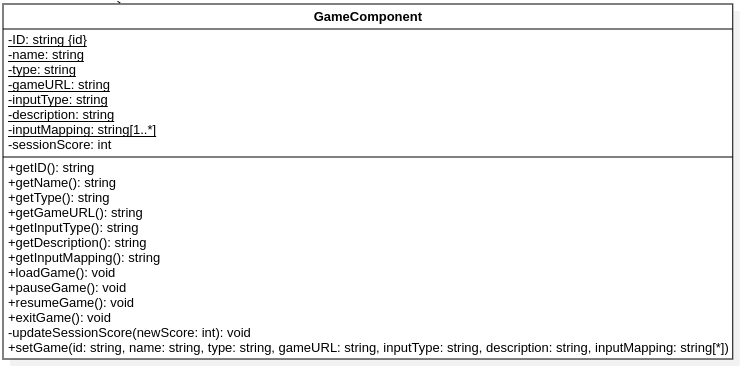
\includegraphics[width=340pt]{images/prog/Game.png}
    \caption{Dettaglio della classe GameComponent}
    \label{fig:gameComponent}
\end{figure}
% immagine dettaglio GameComponent
\emph{GameComponent} rappresenta un gioco all'interno dell'applicativo. Contiene tutte le informazioni necessarie per l'avvio e il controllo dello stesso, oltre alle classiche informazioni "anagrafiche".\\
Un gioco viene rappresentato come:
\begin{itemize}
    \item ID: l'identificativo del gioco, formato da una stringa.
    \item name: nome del gioco.
    \item type: la categoria del gioco.
    \item gameURL: l'indirizzo dove reperire la finestra di gioco, sia locale che remoto.
    \item inputType: la tipologia d'input, tra "controller" e "touchDigit" (ovvero touch/digitalizer).
    \item description: opzionale. Descrizione del gioco, con informazioni generali in merito. Se non sono disponibili, il campo assume valore "not_available".
    \item inputMapping: la mappatura dei controlli da utilizzare per giocare.
\end{itemize}
Inoltre, utilizza \emph{IPCService} per inviare e ricevere eventi inerenti al gioco in esecuzione, e utilizza la variabile sessionScore per registrare il punteggio di gioco più alto durante la sessione.
Infine, i giochi sono memorizzati nel file \emph{games.json}, della cui struttura si parlerà in \nameref{subsec:strutturaFile}. 
\subsubsection{RecordComponent}
\label{subsec:recordComponent}
\begin{figure}[h]
    \centering
    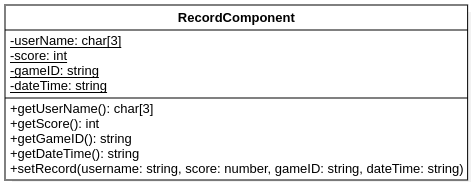
\includegraphics[width=340pt]{images/prog/Record.png}
    \caption{Dettaglio della classe RecordComponent}
    \label{fig:recordComponent}
\end{figure}
% immagine dettaglio RecordComponent
RecordComponent rappresenta un record memorizzato dall'applicativo.\\ Contiene le informazioni relative a un punteggio, effettuato da un determinato utente in un determinato gioco.\\
Un record viene rappresentato come:
\begin{itemize}
    \item userName: il nome dell'utente che ha effettuato un record, formato da un array di tre caratteri.
    \item score: il punteggio eseguito dall'utente.
    \item gameID: l'ID del gioco dove si è effettuato il record.
    \item dateTime: la data e ora di conseguimento del record.
\end{itemize}
I record sono memorizzati nel file \emph{records.json}, della cui struttura si parlerà sempre in \nameref{subsec:strutturaFile}.
\subsubsection{Interfaccia di gioco}
\begin{figure}[h]
    \centering
    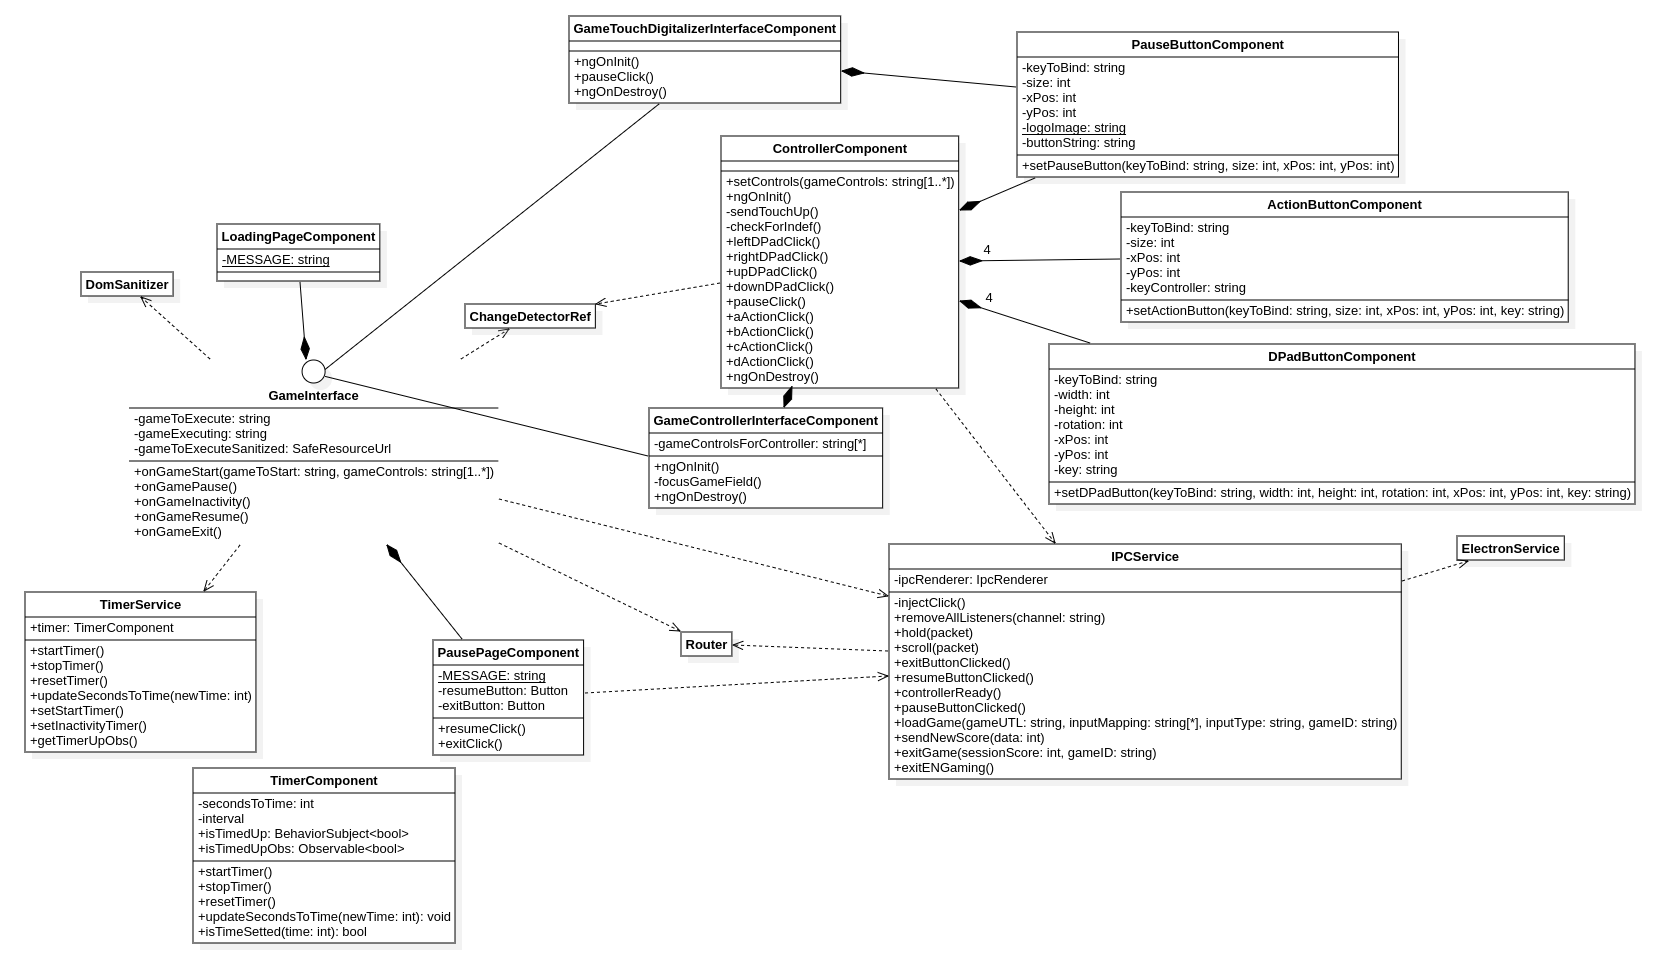
\includegraphics[width=340pt]{images/prog/GameInterface.png}
    \caption{Diagramma delle classi per l'interfaccia di gioco}
    \label{fig:gameinterface}
\end{figure}
% immagine dettaglio Interfaccia di gioco
Dovendo implementare due tipologie di gioco, dev'essere necessario poter creare due interfacce separate, che abbiano però elementi in comune.\\
Per questo motivo, viene utilizzata l'interfaccia \emph{GameInterface}, che contiene il necessario per la corretta visualizzazione del gioco.\\
In particolare, utilizza:
\begin{itemize}
    \item \emph{TimerComponent}, attraverso \emph{TimerService}, per la gestione della schermata di caricamento e lo stato d'inattività.
    \item \emph{LoadingPageComponent} per la visualizzazione della schermata di caricamento.
    \item \emph{PausePageComponent} per visualizzare l'informazione dello stato di pausa del gioco, con le possibilità di riprenderlo o di uscire dallo stesso.
    \item \emph{IPCService} per le comunicazioni tra componenti.
    \item \emph{Router}, \emph{DomSanitizer} e \emph{ChangeDetectorRef}, per i motivi elencati in \nameref{subsec:angularServices}.
\end{itemize}
Questa interfaccia viene implementata da due classi: \emph{GameControllerInterfaceComponent} e \emph{GameTouchDigitalizerInterfaceComponent}.
\newpage
\paragraph{GameControllerInterfaceComponent}
\label{paragraph:gamecontrollerinterfacecomponent}
\emph{GameControllerInterfaceComponent} rappresenta l'interfaccia di gioco per giochi che richiedono l'utilizzo del controller.\\
Questa classe, oltre a essere formata dagli elementi che implementa da \emph{GameInterface}, è formata da un controller. Il controller è composto da:
\begin{itemize}
    \item Quattro \emph{DPadButtonComponent}, che rappresentano i pulsanti per il movimento all'interno del gioco.
    \item Quattro \emph{ActionButtonComponent}, che rappresentano i pulsanti per le azioni\\ all'interno del gioco.
    \item Un \emph{PauseButtonComponent} per mettere in pausa il gioco.
\end{itemize}
Il controller viene configurato, prima dell'avvio, secondo i comandi previsti per il singolo gioco. Se uno o più pulsanti non vengono configurati per un determinato gioco, essi vengono rimossi dalla visualizzazione, al fine di non creare confusione durante l'utilizzo del gioco.\\
Infine, essendo il device target posizionato in un determinato modo, il layout è configurato in maniera da facilitarne l'utilizzo senza prendere in mano il device.\\
In particolare, gli \emph{ActionButtonComponent} presenti sono posizionati in modo da risultare il più possibilmente comodi per questa posizione, ispirandosi alla posizione della mano destra di un pianista.
Un layout di esempio, adatto per questi vincoli, è nell'immagine seguente:
\begin{figure}[h]
    \centering
    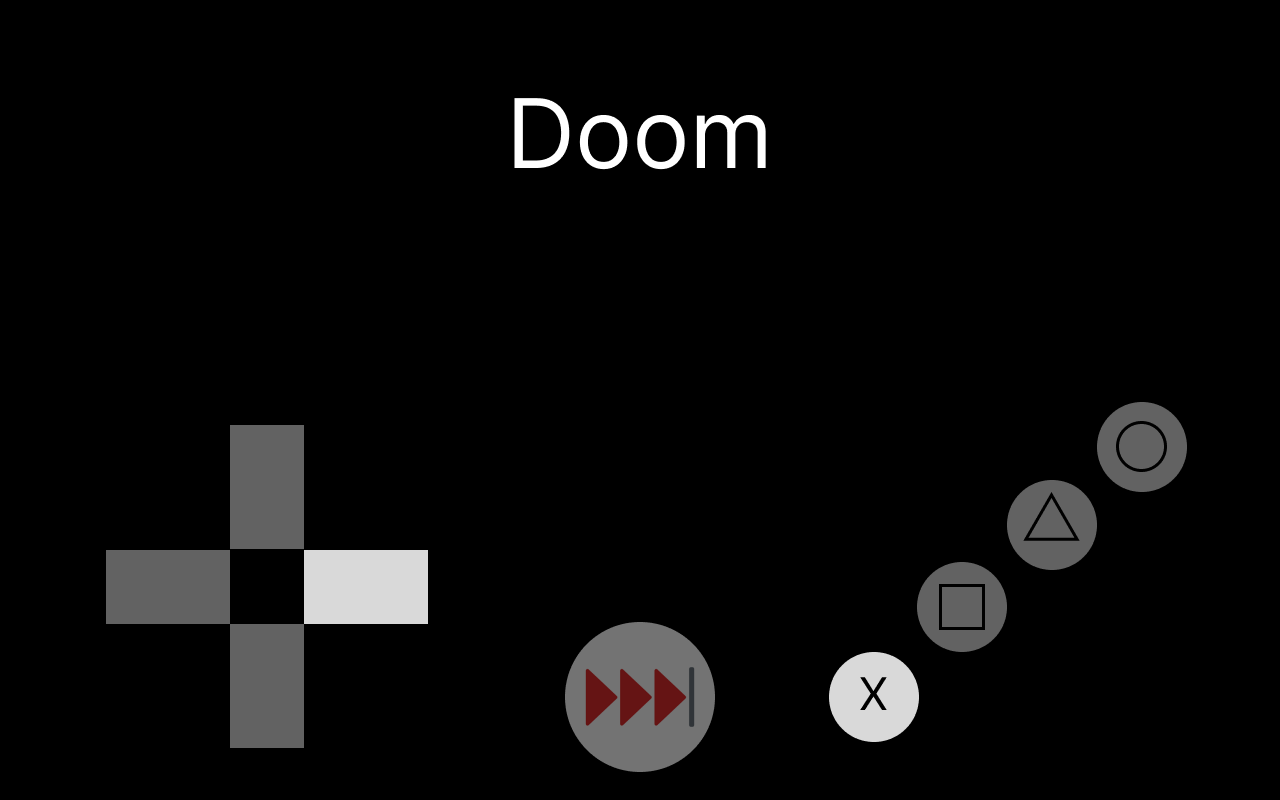
\includegraphics[width=340pt]{images/prog/ControllerMockup.png}
    \caption{Prototipo dell'interfaccia per giochi che richiedono l'uso del controller}
    \label{fig:controller}
\end{figure}
% immagine mockup controller
\paragraph{GameTouchDigitalizerInterfaceComponent}
\emph{GameTouchDigitalizerInterfaceComponent} rappresenta l'interfaccia di gioco per giochi che richiedono l'utilizzo del touch, oppure l'utilizzo del digitalizer.\\
Si noti come in questa classe non si richiede all'utente se scegliere un input tramite il sistema touch o tramite il digitalizer. Questa scelta permette all'utente di utilizzare la modalità che più preferisce, senza vincolarlo.\\
Oltre a essere formata dagli elementi che implementa da \emph{GameInterface}, la classe è formata da un \emph{PauseButtonComponent} per mettere in pausa il gioco.\\
Il \emph{PauseButtonComponent} viene posizionato in alto a destra, poichè l'obiettivo è d'invadere il meno possibile lo spazio di gioco, in modo da non arrecare disturbo durante il gioco.\\
La visualizzazione di tale layout è presente nella seguente figura:
\begin{figure}[h]
    \centering
    
\includegraphics[width=340pt]{images/prog/TouchDigitMockup.png}
    \caption{Prototipo dell'interfaccia per giochi che richiedono l'uso di touch/digitalizer}
    \label{fig:touchDigit}
\end{figure}
% immagine mockup touch/digitalizer
\newpage
\subsubsection{Schermata di salvataggio record}
\begin{figure}[h]
    \centering
    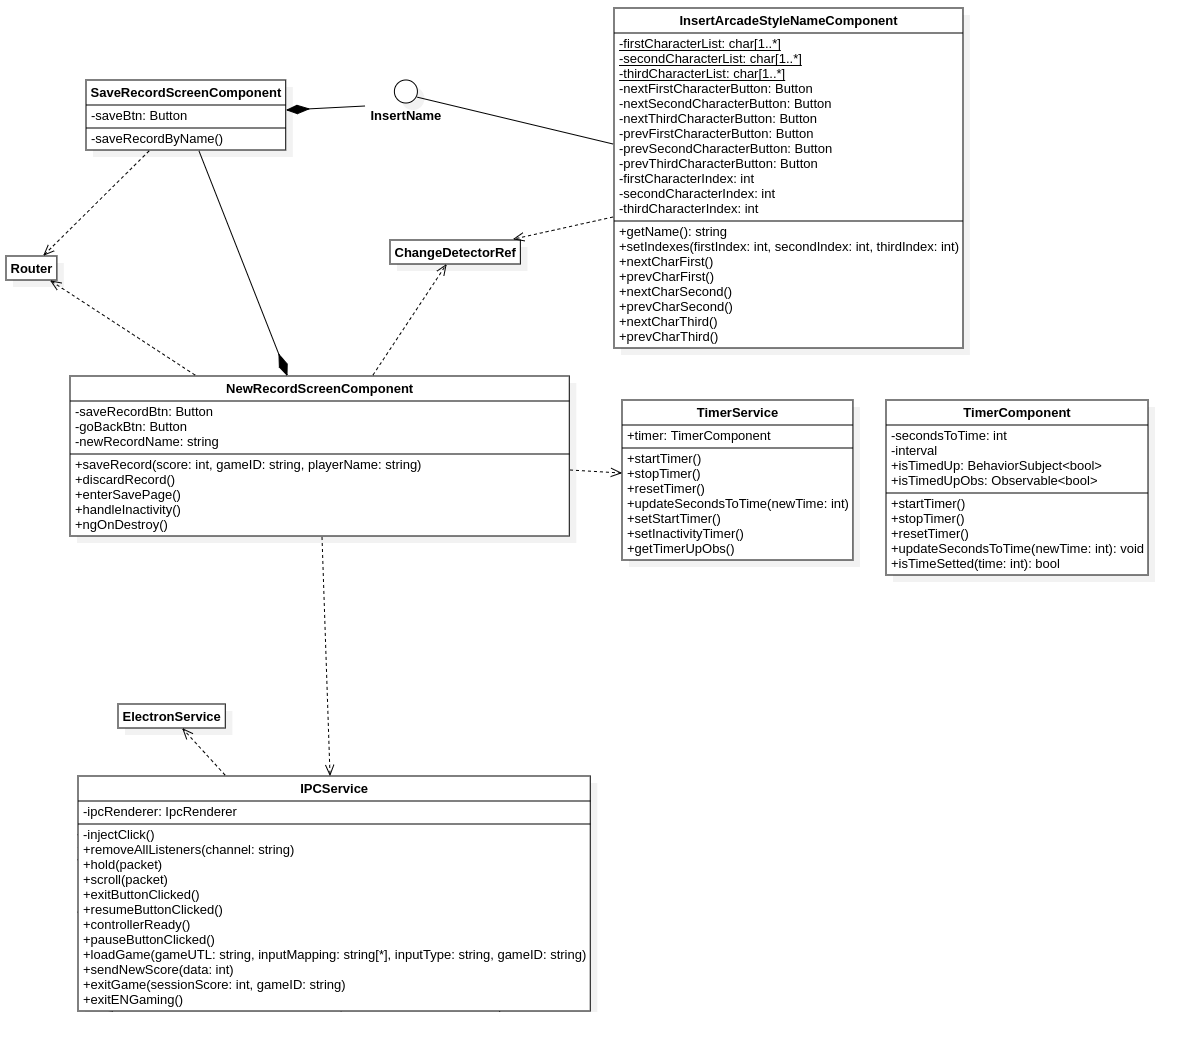
\includegraphics[width=340pt]{images/prog/NewRecord.png}
    \caption{Diagramma delle classi per il salvataggio dei record}
    \label{fig:newRecord}
\end{figure}
% immagine dettaglio salvataggio record
Alla notifica di un nuovo record, viene visualizzata la pagina \emph{NewRecordScreenComponent}, dove viene chiesto all'utente se desidera salvare il record appena effettuato o non salvarlo.\\
Nel caso di salvataggio del record, si passa alla pagina \emph{SaveRecordScreenComponent}, utilizzando un \emph{Router}, che si occupa di ricevere il nome dell'utente. Per far ciò, si avvale della classe \emph{InsertArcadeStyleNameComponent}.\\
Tale classe, che implementa l'interfaccia \emph{InsertName}, prevede l'inserimento dei tre caratteri che compongono il nome utente scegliendo tra i caratteri disponibili, utilizzando gli appositi bottoni.\\
\emph{SaveRecordScreenComponent} inoltre utilizza anche \emph{TimerComponent} attraverso \emph{TimerService} per la gestione dell'inattività in quella determinata schermata.
\newpage
\subsubsection{TimerComponent}
\begin{figure}[h]
    \centering
    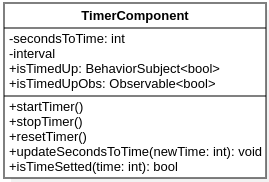
\includegraphics[width=200pt]{images/prog/TimerComponent.png}
    \caption{Dettaglio della classe TimerComponent}
    \label{fig:timer}
\end{figure}
% immagine dettaglio TimerComponent
\emph{TimerComponent}, servito in altri componenti attraverso \emph{TimerService}, si occupa della gestione del tempo.\\ 
Il suo scopo è, dato un tempo espresso in millisecondi, d'iniziare il conteggio, e notificare quando il tempo ha raggiunto la fine.\\
Per far questo, imposta un intervallo della durata memorizzata, notificando tramite un \emph{Observable} quando scade.
\subsubsection{Gestione ENSign11}
\begin{figure}[h]
    \centering
    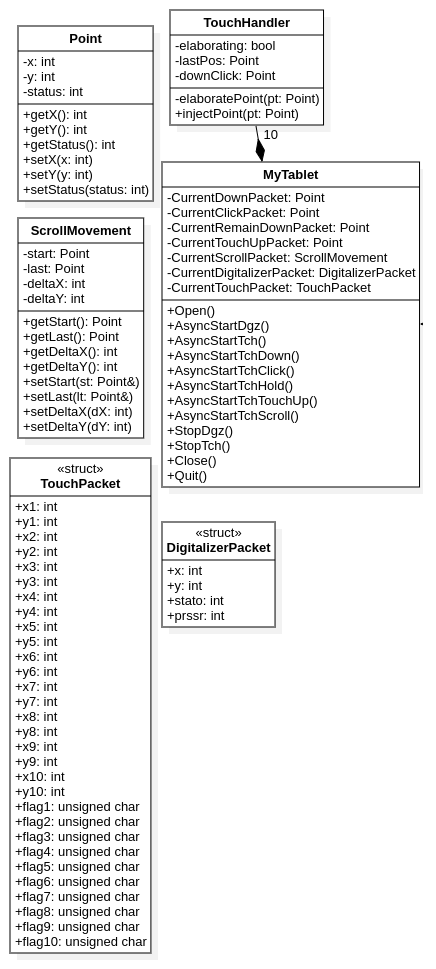
\includegraphics[width=115pt]{images/prog/ENS11.png}
    \caption{Diagramma per la gestione dell'input da ENSign11}
    \label{fig:es11}
\end{figure}
% immagine dettaglio gestione ENSign11
Il device di firma, ovvero l'ENSign11, fornisce le funzioni per interagire con lo stesso attraverso una classe, chiamata \emph{MyTablet}.\\
Questa classe permette l'interazione con il device, come l'apertura e la chiusura dello stesso. Inoltre, offre le funzioni per ottenere gli input dallo stesso.\\
Per il recupero dell'input dal device ENSign11, \emph{MyTablet} si serve della classe \emph{TouchHandler} per il recupero di eventi click, hold, scroll...\\
Questa classe, della quale \emph{MyTablet} ha dieci istanze (una per ogni possibile iterazione, per un massimo di dieci tocchi in contemporanea), rileva se quanto avviene sullo schermo rientra tra i seguenti eventi:
\begin{itemize}
    \item \textbf{Down}: il primo pacchetto che il driver "emette", indica che il dito è stato appena appoggiato sullo schermo.
    \item \textbf{Click}: indica che il dito è stato appoggiato sullo schermo per un breve periodo di tempo.
    \item \textbf{Scroll}: indica che il dito è ancora appoggiato sullo schermo, ma le sue coordinate hanno superato la tolleranza (impostata per evitare falsi movimenti).
    \item \textbf{Hold}: indica che il dito è ancora appoggiato sullo schermo.
    \item \textbf{Touch Up}: l'ultimo pacchetto che il driver "emette", indica che il dito è stato sollevato dallo schermo.
\end{itemize}
I punti, rappresentati da oggetti, che \emph{MyTablet} manda attraverso gli appositi metodi sono:
\begin{itemize}
    \item \textbf{Point}: oggetto che contiene le coordinate del punto e lo stato. Questo oggetto viene mandato per gli eventi elencati prima, a eccezione dell'evento \textbf{Scroll}, durante i giochi che richiedono l'uso del controller e nell'utilizzo generale dell'applicativo.
    \item \textbf{ScrollMovement}: oggetto che contiene i punti (attraverso oggetti \emph{Point}) d'inizio e fine del movimento, e le variazioni delle coordinate x e y. Questo oggetto viene mandato per l'evento \textbf{Scroll}.
    \item \textbf{TouchPacket}: oggetto che contiene le coordinate e lo stato di tutti e dieci i tocchi. L'oggetto viene inviato durante l'esecuzione di giochi che non richiedono l'uso del controller.
    \item \textbf{DigitalizerPacket}: oggetto che contiene le coordinate, lo stato del digitalizer e la pressione applicata dall'utente. L'oggetto viene inviato durante l'esecuzione di giochi che non richiedono l'uso del controller.
\end{itemize}
\subsubsection{Servizi di Angular}
\label{subsec:angularServices}
ENGaming utilizza i seguenti servizi, offerti da Angular, per l'esecuzione del programma:
\begin{itemize}
    \item \textbf{Router}: permette di essere reindirizzati da un componente a un altro, aggiornando la vista, tramite il metodo \emph{navigate}.
    \item \textbf{ChangeDetectorRef}: aggiorna la vista tramite il metodo \emph{detectChanges}.
    \item \textbf{ActivatedRoute}: permette di recuperare l'URL della pagina in cui ci si trova.
    \item \textbf{ElectronService}: permette l'utilizzo dei canali IPC e delle funzioni generalmente presenti in Electron.
    \item \textbf{DomSanitizer}: effettua il processo di "pulizia" di un URL, permettendo la visualizzazione del suo contenuto in un elemento \emph{iframe} oppure \emph{object}.
\end{itemize}
\subsection{Struttura dei file utilizzati}
\label{subsec:strutturaFile}
Come indicato in \nameref{subsec:gameComponent} e \nameref{subsec:recordComponent}, vengono utilizzati due file json, il primo contiene le informazioni sui giochi (\emph{games.json}), il secondo contiene i record effettuati (\emph{records.json}).
\subsubsection{Games.json}
Il file, che viene aperto da ENGaming solamente in lettura, contiene le informazioni necessarie dei giochi e delle loro relative pagine. Ne consegue che la modifica di questo file debba essere fatta manualmente.\\
Un esempio di giochi presenti nel file è il seguente:
\begin{lstlisting}[language=json,firstnumber=1]
    [
        {
            "id": "catMario",
            "name": "Cat Mario",
            "type": "Azione",
            "gameURL": "https://www.cat-mario.com/",
            "inputType": "controller",
            "description": "Clone di Super Mario, con un gatto. Per nulla stressante!",
            "inputMapping": [
                "salto:A:Space",
                "muovi a sinistra:DPad Left:Left",
                "muovi a destra:DPad Right:Right"
            ]
        },
        {
            "id": "subwaySurfers",
            "name": "Subway Surfers",
            "type": "Endless",
            "gameURL": "src_angular/assets/games/subwaySurfers/index.html",
            "inputType": "touchDigit",
            "description": "not_available",
            "inputMapping": [
                "inizia: tap",
                "muovi a sinistra: swipe a sinistra",
                "muovi a destra: swipe a destra",
                "salto: swipe in alto",
                "rotolata:swipe in basso"
            ]
        }
    ]
\end{lstlisting}
Dove i giochi con il controller richiedono anche la conoscenza dei tasti che il gioco richiede tramite l'utilizzo della tastiera.\\
Inoltre, i giochi possono essere caricati con i sorgenti tramite il percorso relativo degli stessi.
\newpage
\subsubsection{Records.json}
Il file contiene tutti i record effettuati nell'applicativo. Tale file non è condiviso in rete ed è unico per ogni installazione. Quindi, i record possono variare da una macchina a un'altra.\\
Questo è l'unico file che viene caricato da ENGaming sia per la lettura che per la scrittura, non richiedendo una scrittura manuale dei dati.\\
Un esempio di record che il file contiene è il seguente:
\begin{lstlisting}[language=json,firstnumber=1]
    [
        {
            "userName": "AAA",
            "score": "250",
            "gameID": "dukeNukem",
            "dateTime":"2024-02-15 17:23"
        },
        {
            "userName": "RIC",
            "score": "420",
            "gameID": "angryBirds",
            "dateTime":"2024-05-19 08:23"
        }
    ]
\end{lstlisting}
\subsection{Scelte progettuali}
Oltre a quanto già visto, ho adoperato diverse scelte durante questa fase.\\
In particolare:
\begin{itemize}
    \item architetturalmente, ho scelto di utilizzare il modello Model-View-ViewModel (abbreviato MVVM), in quanto tra le possibili architetture l'ho ritenuta la più adatta per il progetto.
    \item l'utilizzo di \Gls{angl} mi consente di ridurre l'accoppiamento per componenti attraverso l'utilizzo della \emph{Dependency Injection} per l'utilizzo dei servizi.
    \item l'utilizzo degli \Gls{ipcg} mi permettono di far comunicare gli elementi che compongono l'applicazione, in particolare tra le classi implementate in \Gls{angl} ed \Gls{elctr}, attraverso lo scambio di messaggi in appositi canali.\\Tale comportamento è simile al comportamento di un \emph{Observer}.
    \item per rendere minore la dipendenza tra le componenti, ho scelto di non utilizzare alcun tipo di gerarchia. Questa scelta è dovuta, oltre alla non reale necessità del suo utilizzo, alla limitatezza a livello applicativo, in quanto tra le tecnologie da usare solo \gls{cpp} permette l'uso di una gerarchia.
    \item invece di ricorrere all'utilizzo delle gerarchie, ho scelto di definire le parti comuni attraverso un'interfaccia, che viene poi implementata dalle singole classi che la necessitano.
\end{itemize}
\section{Codifica}
\subsection{Strumenti utilizzati}
Per lo sviluppo di ENGaming, oltre a quanto già citato in \nameref{sec:sviluppoStrum}, ho utilizzato:

\begin{itemize}
    \item NodeJS, versione 18.16.0
    \item Npm, versione 9.5.1
    \item TypeScript, versione 4.9.5
    \item C++,versione 17
    \item AngularCLI, versione 15.2.8
    \item Electron, versione 25.0.1
    \item Git, versione 2.41.0
\end{itemize}
\subsection{Ambiente di sviluppo}
Per tenere una suddivisione chiara delle parti da sviluppare, ho impostato la cartella di lavoro secondo questa struttura:
\begin{itemize}
    \item src_angular \begin{itemize}
        \item app \begin{itemize}
            \item COMPONENTI
            \item <<servizi>>
            \item <<interfacce>>
        \end{itemize}
        \item assets \begin{itemize}
            \item games \begin{itemize}
                \item GIOCHI
            \end{itemize}
            \item previews \begin{itemize}
                \item <<immagini>>
            \end{itemize}
            \item games.json
            \item records.json
            \item <<altri file>>
        \end{itemize}
        \item index.html
        \item main.ts
        \item <<altri file>>
    \end{itemize}
    \item src_electron \begin{itemize}
        \item App.ts
        \item ENGaming.ts
    \end{itemize}
    \item src_module \begin{itemize}
        \item ES11LIB
        \item ES11LOADER
        \item LIBUSB
        \item <<altri file>>
    \end{itemize}
\end{itemize}
Dove:
\begin{itemize}
    \item COMPONENTI indica le cartelle di tutti i componenti, di cui la struttura si è precedentemente illustrata in \nameref{subsec:angular}.
    \item <<servizi>> indica i file dei servizi, che sono dotati solo di un file Typescript per la definizione dei comportamenti.
    \item <<interfacce>> indica i file delle interfacce, dotati solo di un file Typescript per la definizione delle stesse.
    \item GIOCHI indica le cartelle dove sono presenti i giochi, con i relativi sorgenti.
    \item <<immagini>> indica le immagini utilizzate dall'applicativo.
    \item ES11LIB indica la cartella che contiene i driver per il funzionamento dell'ENSign11, ricevuti direttamente dall'azienda.
    \item ES11LOADER indica la cartella dove risiedono i file per la gestione dell'ENSign11, ai quali ho personalmente lavorato.
    \item LIBUSB indica la cartella dove risiede la libreria usata dai file contenuti in ES11LIB.
    \item <<altri file>> indica altri file, presenti nelle cartelle ma di minore interesse (ad esempio, file .gitignore)
\end{itemize}
Nello stesso livello delle cartelle principali, sono presenti anche i file di configurazione, in particolare i file \emph{package.json},\emph{angular.json}, \emph{tsconfig.json} e \emph{forge.config.js}.\\
Il progetto, durante il suo sviluppo, è stato versionato e caricato su una repository, presente in AWS.
\newpage
\subsection{Utilizzo dell'applicativo}
Alla fine della fase di codifica, assistito dal tutor, ho creato gli eseguibili (installers oppure pacchetti, a seconda della piattaforma), attraverso \Gls{elctrForge}.
Allo stato da me raggiunto, ENGaming può essere utilizzato con:
\begin{itemize}
    \item un PC con installato il driver \gls{displaylink} e uno dei seguenti sistemi operativi: \begin{itemize}
    \item Windows 11\footcite{site:w11} (non necessario installare il driver citato in precedenza, in quanto già presente);
    \item MacOS Ventura\footcite{site:macosVentura}.
    \end{itemize}
    \item un ENSign11\footcite{site:ensign11} da collegare a suddetto PC.
\end{itemize}
Purtroppo non ho potuto testare l'applicativo in altre versioni di Windows o MacOS, a causa della mancanza di tempo nel farlo. Non sono invece stati testati altri device di firma poichè non sono stati considerati come device target, a differenza dell'ENSign11.
Su sistemi operativi con kernel Linux, l'applicativo veniva eseguito ma non riconosceva il tablet, costringendo un utilizzo tramite tastiera e mouse e in generale con errori dovuti proprio al non riconoscimento del device.
\newpage
\subsection{Panoramica del prodotto}
\label{subsec:panoramicaProdotto}
Per concludere questa sezione, voglio mostrare il frutto della fase di codifica, partendo dalla schermata iniziale e concludendo con la gestione dell'inattività.
\subsubsection{Schermata iniziale}
La schermata iniziale dell'applicazione comprende:
\begin{itemize}
    \item Il nome dell'applicazione stessa;
    \item L'elenco dei giochi disponibili, sotto forma d'icone;
    \item Un'icona per visualizzare i record effettuati;
    \item Un'icona per uscire dall'applicazione.
\end{itemize}
\begin{figure}[h]
    \centering
    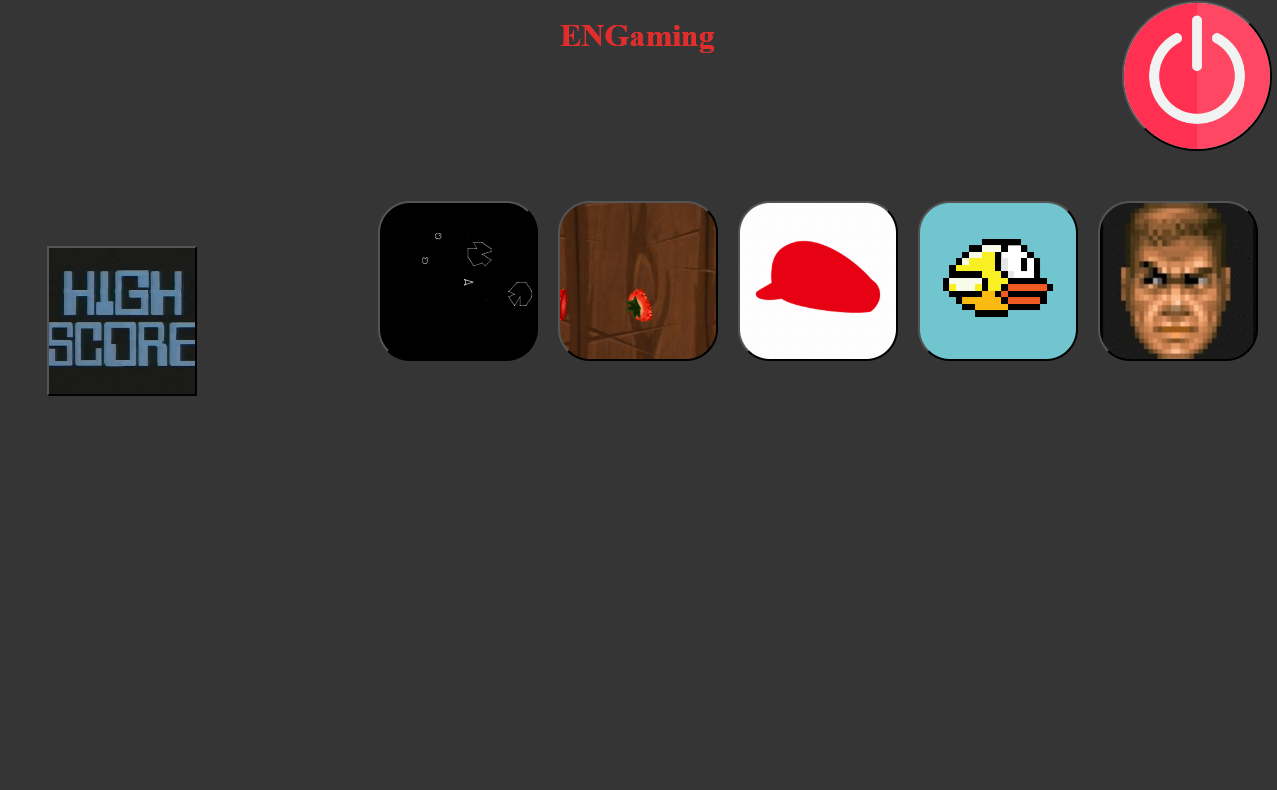
\includegraphics[width=250pt]{images/product/schermataIniziale.png}
    \caption{Schermata iniziale di ENGaming}
    \label{fig:schermataIniziale}
\end{figure}
Ho scelto una visualizzazione il più possibile vicina alle icone per portare un senso di famigliarità, in quanto ENGaming viene usato attraverso uno schermo touch.
\newpage
\subsubsection{Visualizzazione record}
Attraverso l'icona "High Score", è possibile passare alla visualizzazione dei record.
La pagina apposita mostra la lista dei record globale, ovvero mostra tutti i record effettuati senza distinzione di gioco.\\
In particolare, ogni record mostra:
\begin{itemize}
    \item l'utente che ha effettuato il record;
    \item il punteggio totalizzato;
    \item la data in cui è stato effettuato il record;
    \item il gioco in cui è stato effettuato il record.
\end{itemize}
\begin{figure}[h]
    \centering
    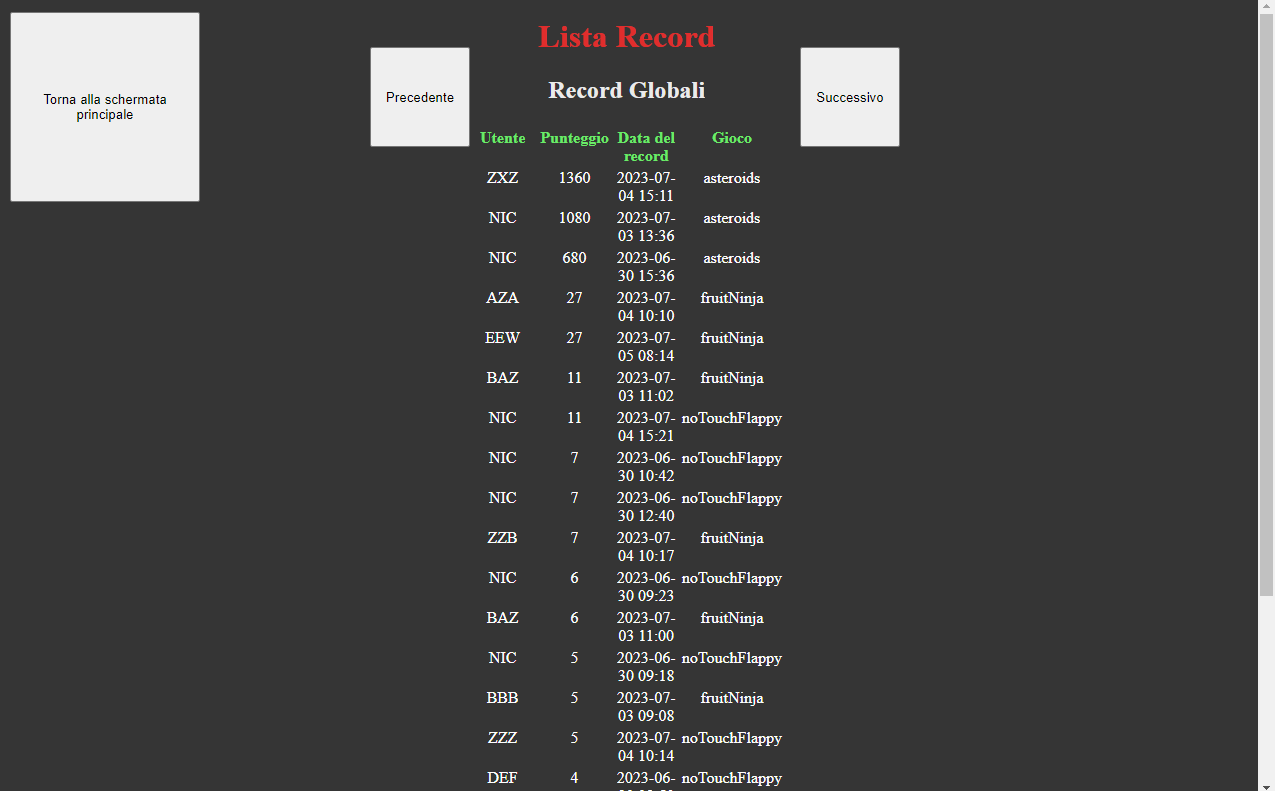
\includegraphics[width=225pt]{images/product/schermataRecord.png}
    \caption{Lista dei record globali}
    \label{fig:schermataRecord}
\end{figure}
Utilizzando i pulsanti "attorno" alla lista, si può passare alla lista dei record per i giochi specifici.
Tali liste sono tante quanti i giochi in cui sia stato fatto almeno un record.
La prima e l'ultima lista di questo genere, alla pressione degli appositi pulsante, riportano alla lista globale.
\begin{figure}[h]
    \centering
    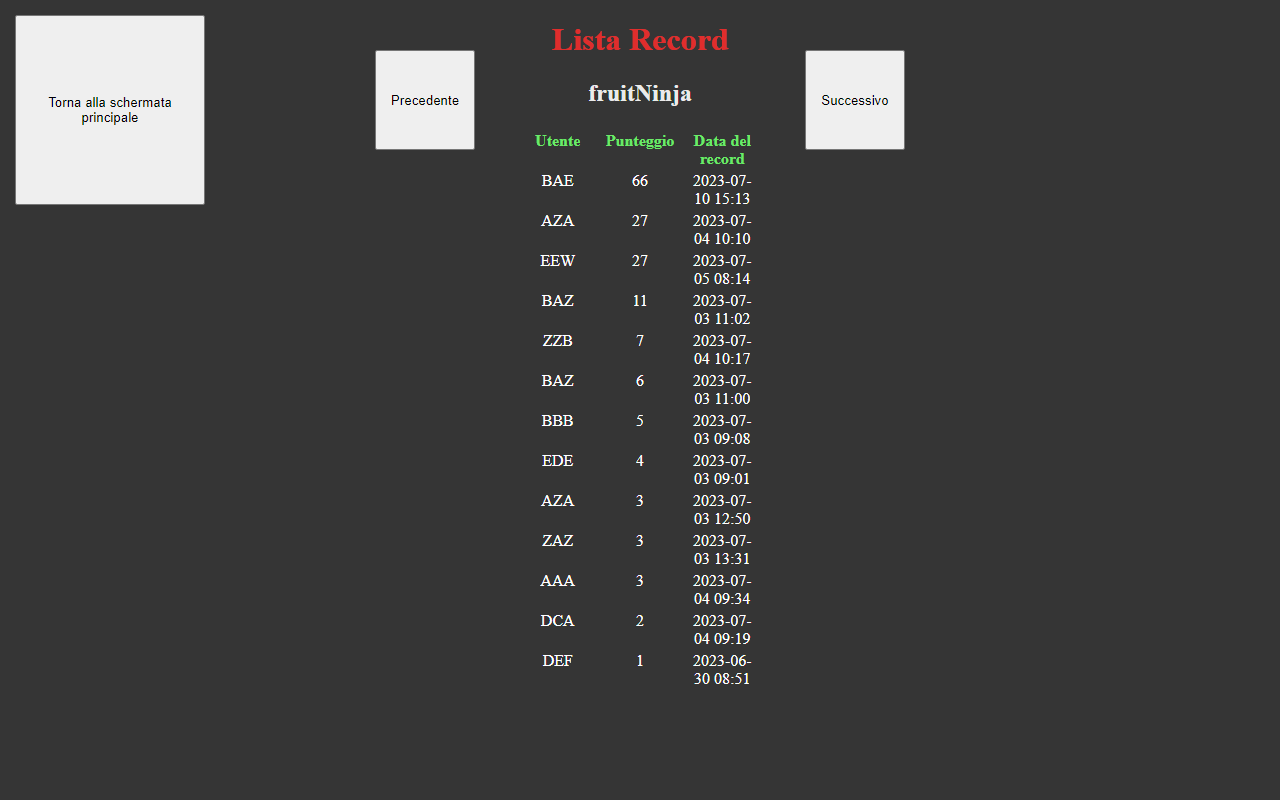
\includegraphics[width=225pt]{images/product/schermataRecordSingoloGioco.png}
    \caption{Esempio di lista per un singolo gioco}
    \label{fig:schermataRecordSingoloGioco}
\end{figure}
\newpage
\subsubsection{Pagina di gioco}
Ritornando alla schermata iniziale, si può selezionare un gioco attraverso la propria icona.
Tale operazione porta alla pagina del gioco stesso, che contiene le informazioni sul gioco stesso, ovvero:
\begin{itemize}
    \item il nome del gioco;
    \item il genere del gioco;
    \item il tipo d'input, ovvero se viene utilizzato il controller o il touch/digitalizer;
    \item la descrizione del gioco;
    \item L'elenco degli input, o delle gesture, che il gioco ha.
\end{itemize}
\begin{figure}[h]
    \centering
    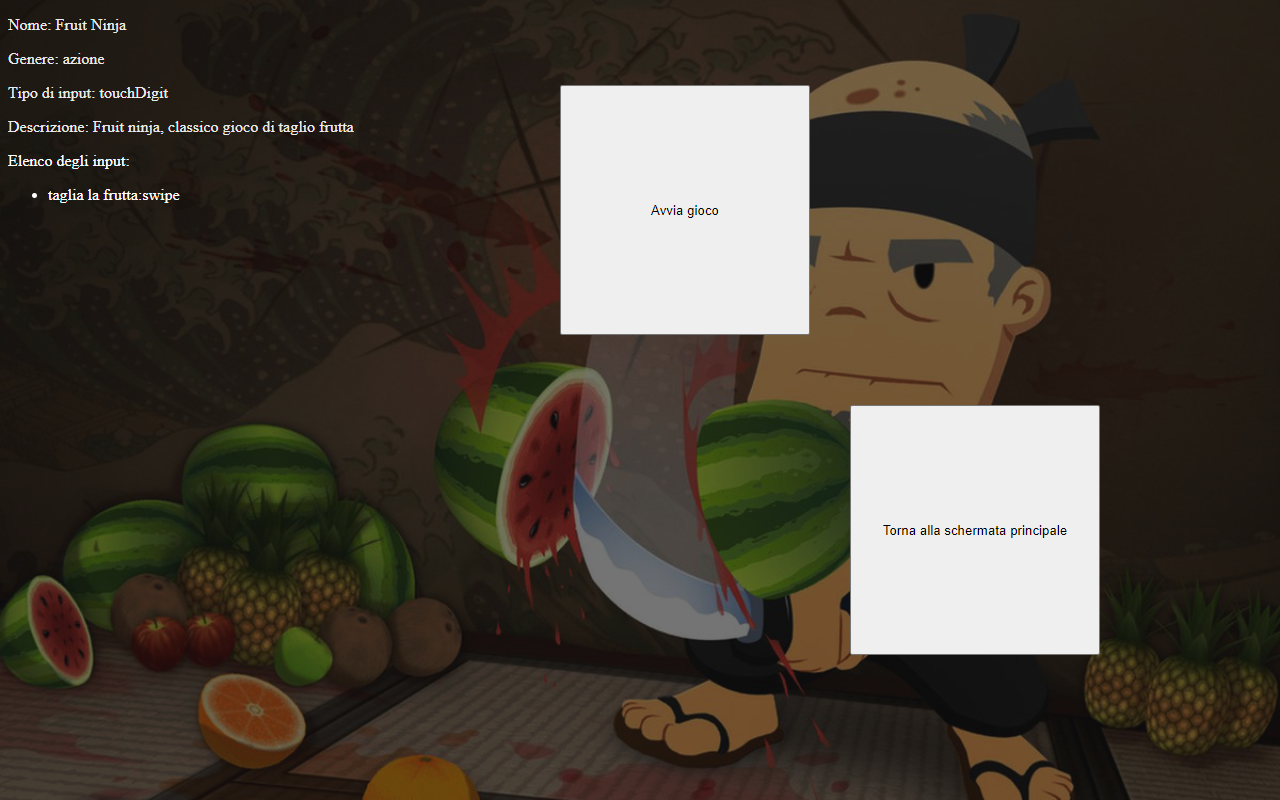
\includegraphics[width=250pt]{images/product/schermataPaginaGioco.png}
    \caption{Esempio di pagina di un gioco}
    \label{fig:schermataPaginaGioco}
\end{figure}
Ovviamente, da questa pagina si può decidere se avviare il gioco o tornare alla schermata principale.
\newpage
\subsubsection{Schermata di caricamento}
All'avvio del gioco, si passa attraverso una pagina di caricamento. La pagina in questione è spoglia, in quanto informa semplicemente l'utente dello stato di caricamento.
Questa pagina viene visualizzata per quattro secondi, per poi passare all'interfaccia di gioco.
\begin{figure}[h]
    \centering
    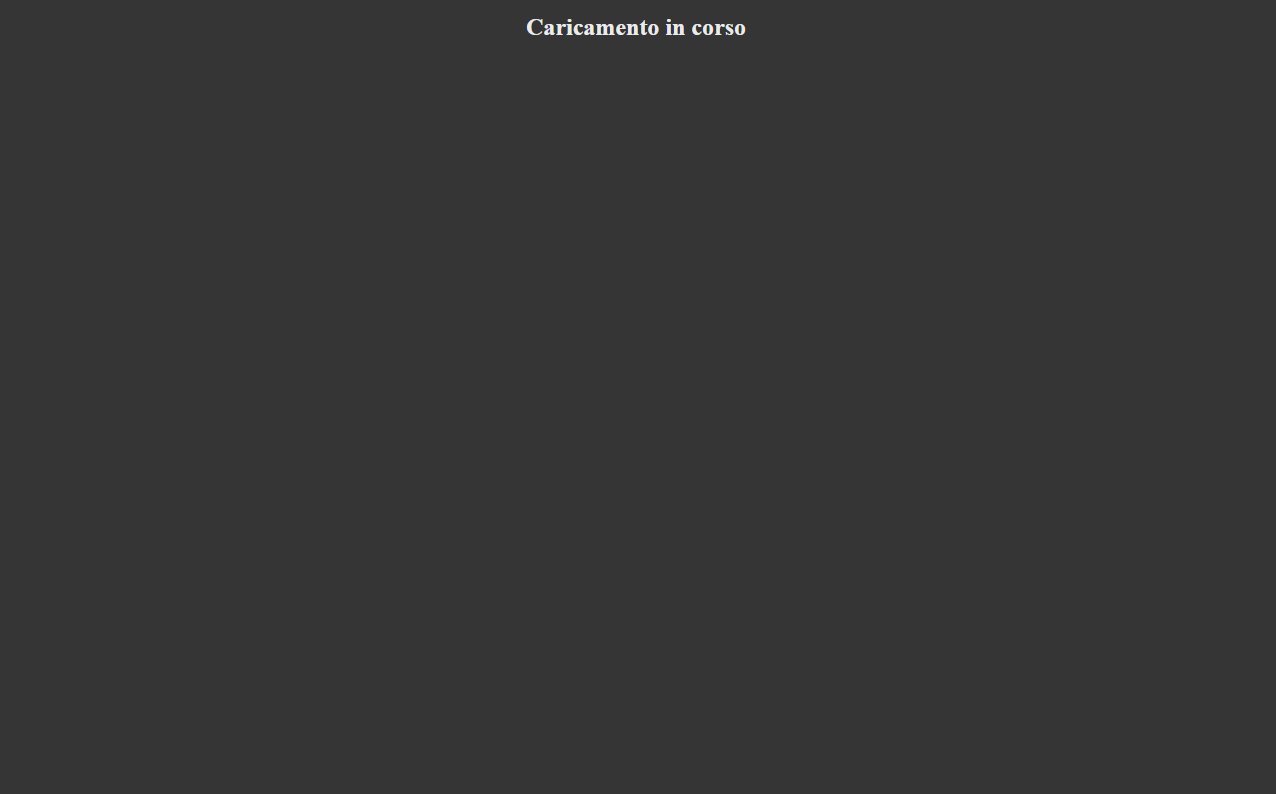
\includegraphics[width=250pt]{images/product/schermataCaricamento.png}
    \caption{Schermata di caricamento}
    \label{fig:schermataCaricamento}
\end{figure}

\subsubsection{Schermate di gioco}
La differenza tra le due tipologie di gioco entra adesso.
Infatti, se il gioco prevede l'utilizzo del controller, oltre al gioco stesso si visualizza anche il controller, che dalla struttura di default (spiegata in \nameref{paragraph:gamecontrollerinterfacecomponent}), viene configurato attraverso gli input che il gioco richiede.
\begin{figure}[h]
    \centering
    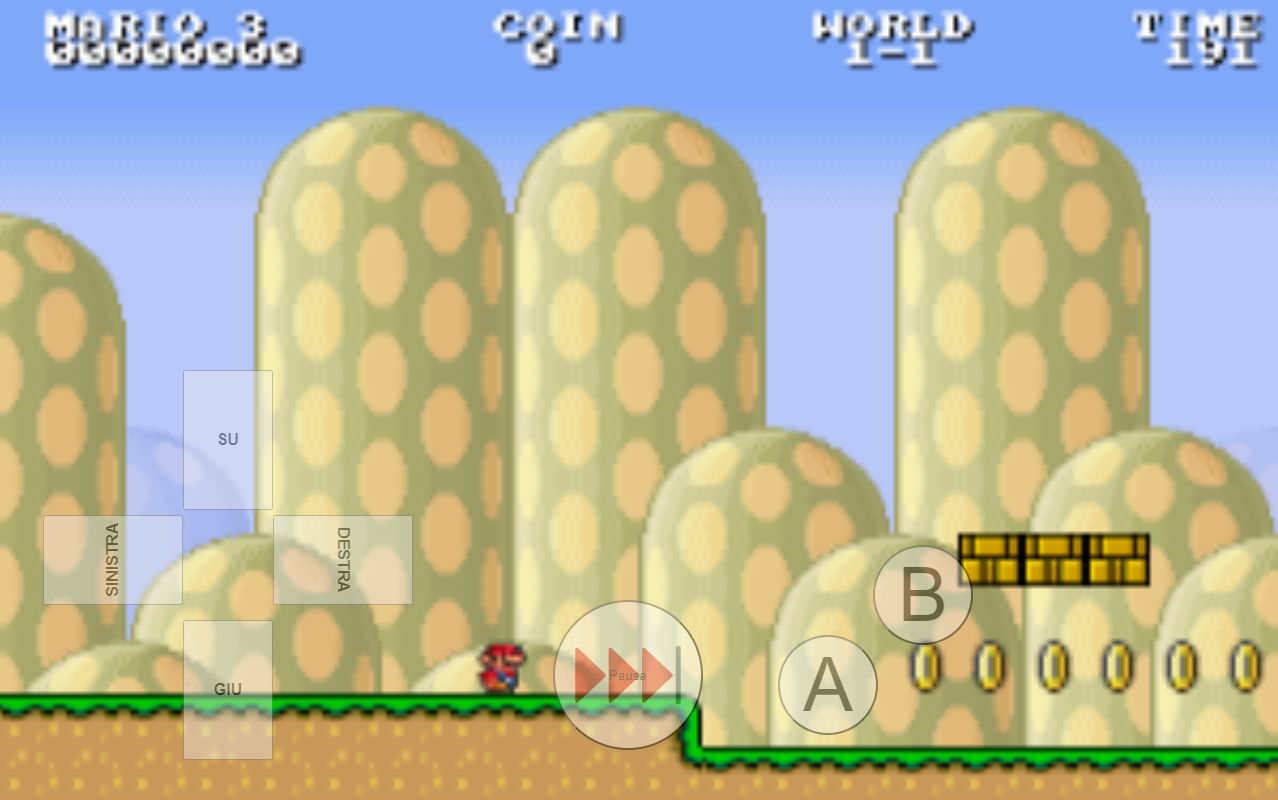
\includegraphics[width=250pt]{images/product/schermataGiocoController.png}
    \caption{Esempio di schermata per un gioco con il controller}
    \label{fig:schermataGiocoController}
\end{figure}
\newpage
Mentre, se il gioco prevede l'utilizzo del touch o del digitalizer, ciò che viene visualizzato sono solo il gioco e il pulsante di pausa, essendo gli input del gioco dati dalle gestures.
\begin{figure}[h]
    \centering
    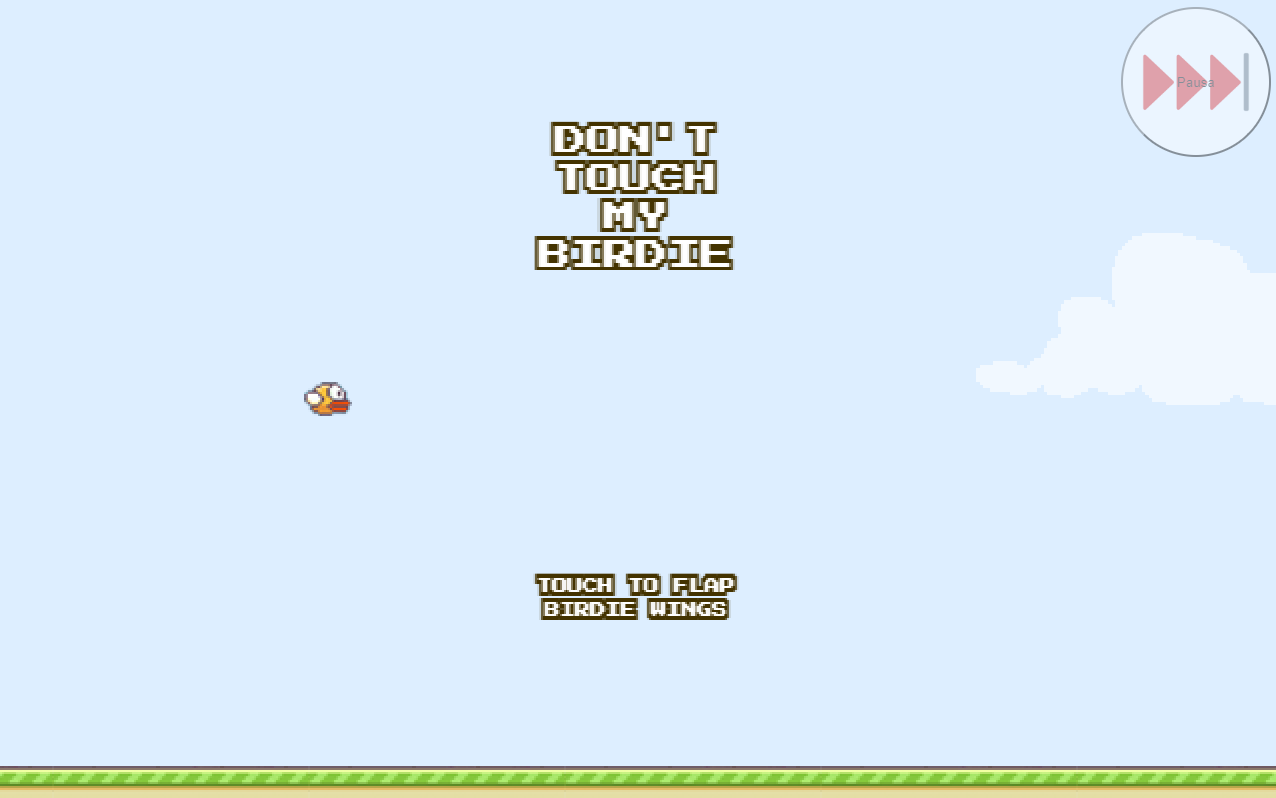
\includegraphics[width=250pt]{images/product/schermataGiocoTouchDigit.png}
    \caption{Esempio di schermata per un gioco con il touch/digitalizer}
    \label{fig:schermataGiocoTouchDigit}
\end{figure}
\subsubsection{Schermata di pausa}
In ogni gioco, a prescindere dal tipo, premendo sul pulsante di pausa si va all'apposita schermata di pausa.
La schermata di pausa informa l'utente dello stato di pausa del gioco, e ne permette la ripresa oppure l'uscita dallo stesso.
\begin{figure}[h]
    \centering
    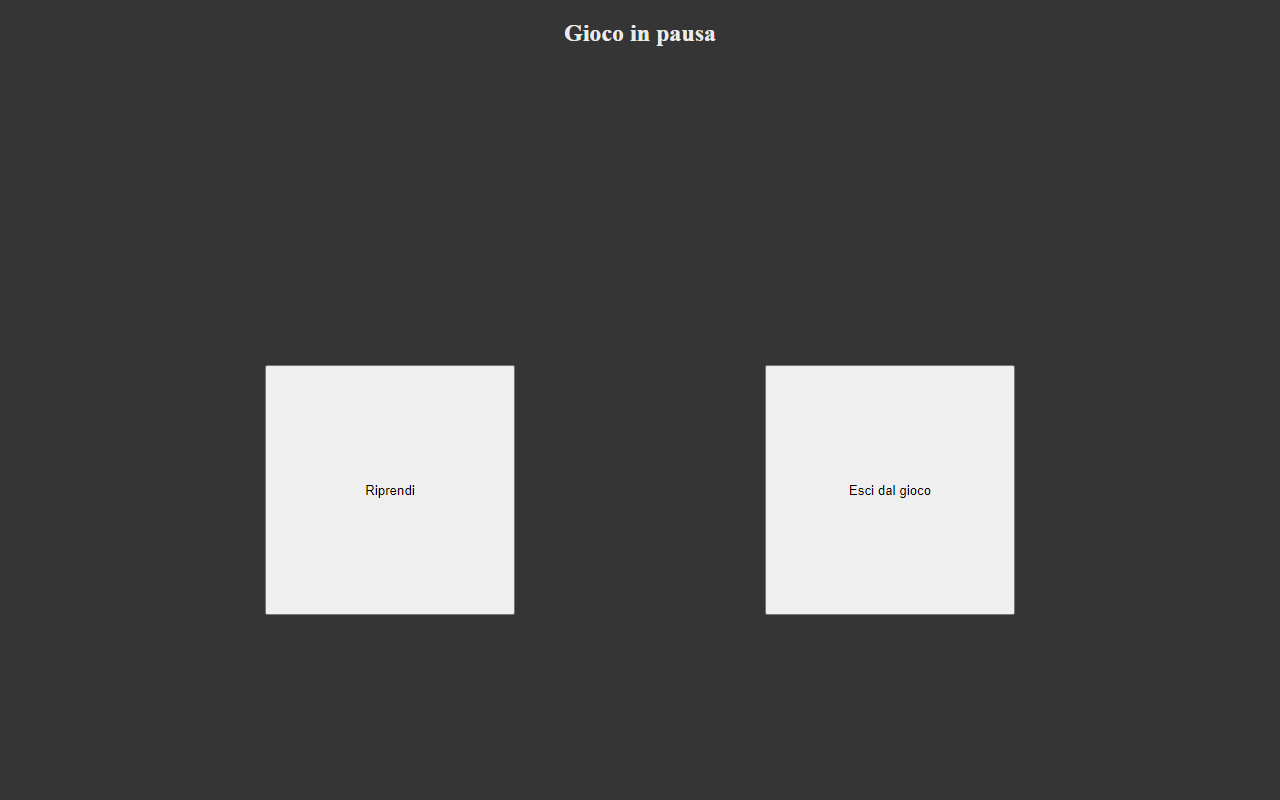
\includegraphics[width=250pt]{images/product/schermataPausaGioco.png}
    \caption{Schermata di pausa}
    \label{fig:schermataPausaGioco}
\end{figure}
\newpage
\subsubsection{Salvataggio record}
Ovviamente una parte importante dell'applicazione è il salvataggio dei record effettuati nei giochi. Per far questo, si passa attraverso due schermate.
La prima informa semplicemente l'utente che ha effettuato un nuovo record nel gioco appena concluso. Oltre a questo, permette allo stesso di decidere se salvarlo o meno.
\begin{figure}[h]
    \centering
    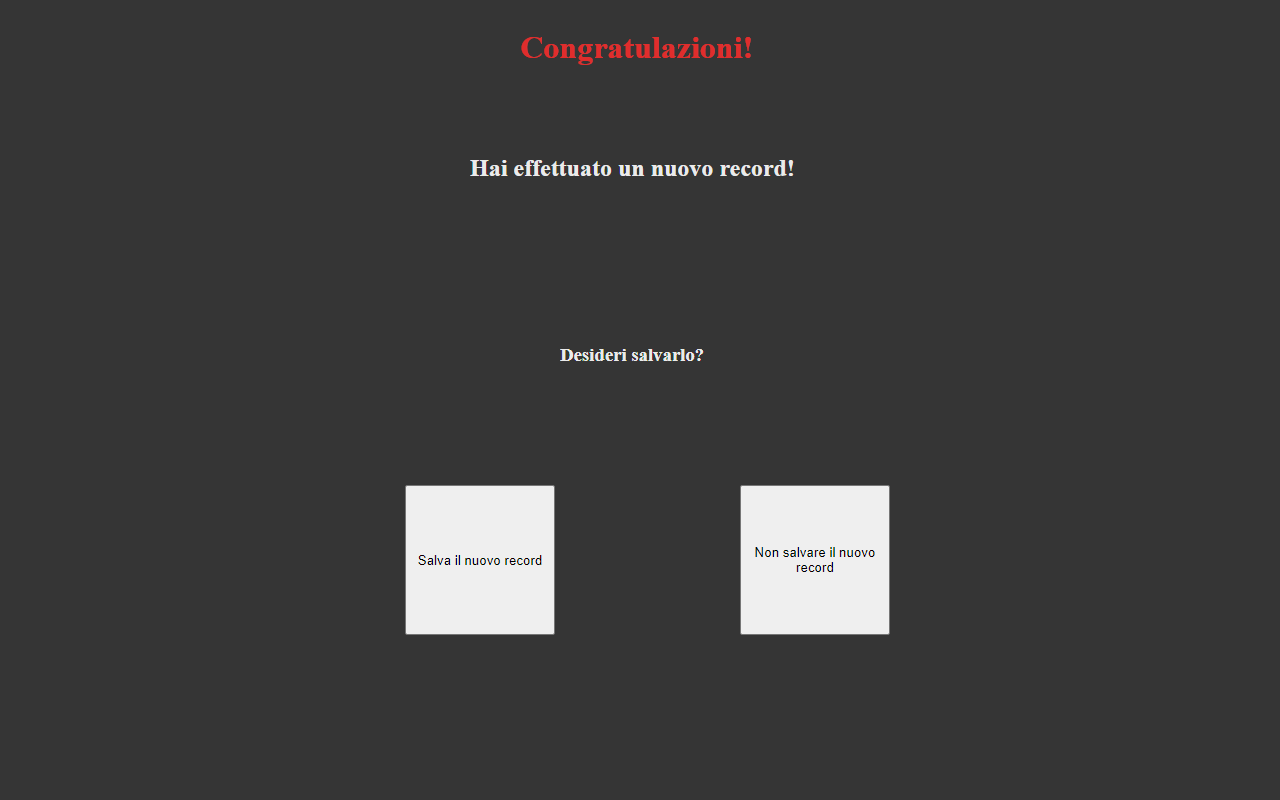
\includegraphics[width=250pt]{images/product/schermataNuovoRecord.png}
    \caption{Schermata di avviso per un nuovo record}
    \label{fig:schermataNuovoRecord}
\end{figure}
\\Nel caso non si voglia salvare il record, l'applicativo semplicemente ritorna nel menù principale, perdendo il punteggio da salvare.
Se invece l'utente vuole salvare il record, viene portato alla seconda schermata, dedicata all'inserimento del nome.\\
Il nome viene inserito attraverso dei pulsanti, che permettono di selezionare, una per volta, le tre lettere che compongono il nome a cui associare il record.
\begin{figure}[h]
    \centering
    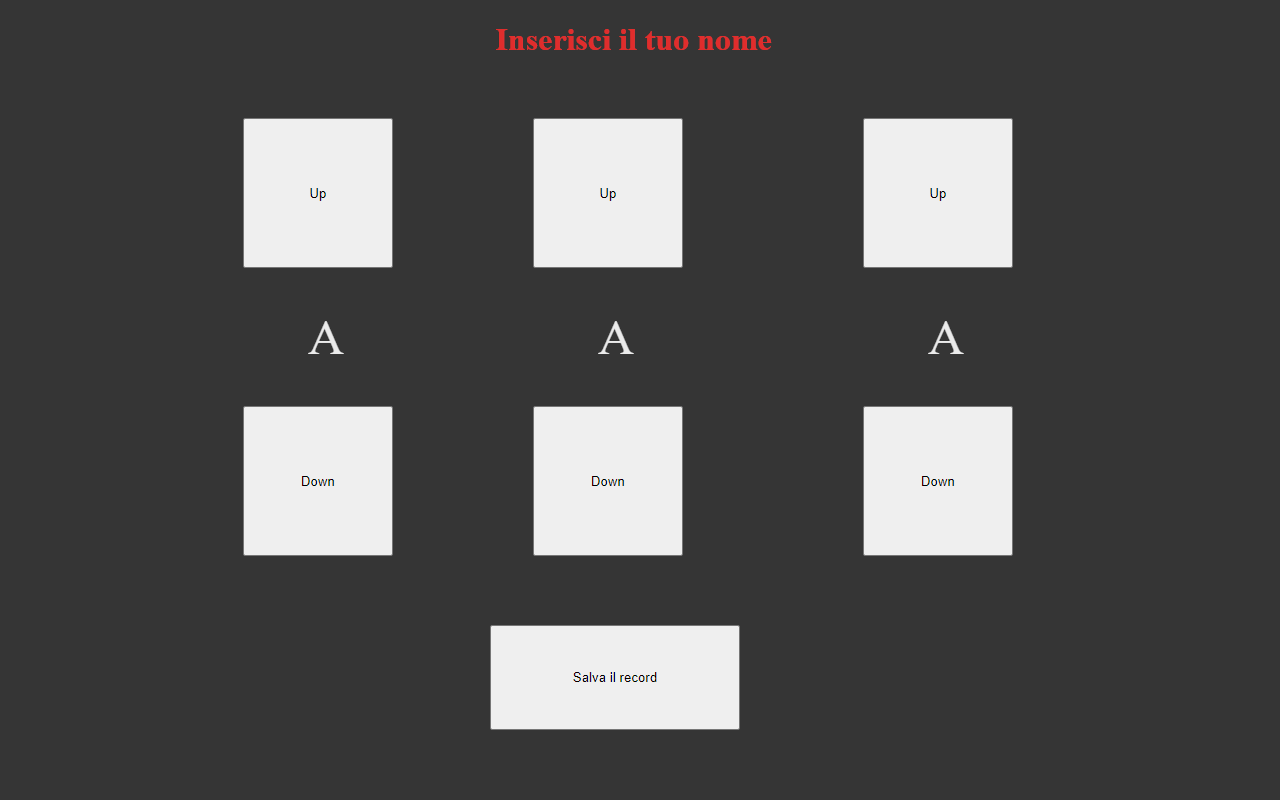
\includegraphics[width=250pt]{images/product/schermataInserimentoNome.png}
    \caption{Schermata per l'inserimento del nome}
    \label{fig:schermataInserimentoNome}
\end{figure}
\\Ho scelto lo stile dei giochi arcade per un principio specifico, ovvero l'inserimento d'input senza dover ricorrere a periferiche esterne a quelle presenti. Infatti, grazie a questa modalità, si può utilizzare lo schermo del device senza incorre in tastiere virtuali o fisiche.
\subsection{Gestione degli errori}
A livello di comportamento, ENGaming prevede pochi casi di errore, essendo un sistema che non prevede configurazioni da parte dell'utente.
Voglio comunque elencare delle piccole accortezze che ho implementato, in quanto si sono rivelate utili anche alla prevenzione di altri errori.
\subsubsection{Gestione del non collegamento del device}
ENGaming, durante l'avvio, cerca d'individuare un ENSign11, in modo da collocarci l'applicazione al suo interno. Nel caso l'utente non colleghi un device prima dell'avvio, l'applicazione riporta un errore all'utente, terminando l'esecuzione del programma.
\subsubsection{Gestione dell'inattività}
\label{sec:inactivity}
L'applicazione, se non rileva alcun input per dieci secondi, fa partire un timer d'inattività della durata massima di quattro minuti. Tale timer si azzera se durante questo lasso di tempo riceve un input.
Nel caso scada il tempo, il sistema chiude l'attività in esecuzione (gioco o salvataggio del record) e ritorna alla schermata principale.
Tale azione comporta la perdita di un eventuale record effettuato e non ancora salvato, in quanto l'attività precedentemente in esecuzione viene chiusa forzatamente.
    \chapter{Verifica e validazione}
\label{cap:verifica-validazione}

Verifica e validazione sono due parti fondamentali dello sviluppo di un software.\\
Il processo di verifica permette di controllare che quanto è prodotto sia effettivamente congruo con i requisiti, attraverso test automatici o manuali.\\
Il processo di validazione permette la convalida di quanto prodotto, secondo quanto precedentemente verificato.\\\\
Per la fase di verifica, per questo progetto, non sono ricorso all'utilizzo di test automatizzati, poiché i casi d'uso e i comportamenti che l'applicativo esegue sono definiti e limitati in quantità.\\
Dunque, ho effettuato la verifica sulle singole parti in maniera manuale, attraverso il debug tramite gli strumenti da me scelti, che hanno reso la stessa poco costosa a livello temporale.\\\\
La fase di validazione è stata fatta assieme al tutor, in due momenti distinti.\\
Infatti, la prima validazione è stata effettuata ancor prima della fase di Analisi, che ha decretato quanto prodotto durante la fase di Formazione Personale come Proof of Concept\footnote{Con Proof of Concept si intende una realizzazione incompleta o abbozzata di un progetto, allo scopo di dimostrarne la fattibilità.}.\\
La seconda (e "vera") validazione ha coinvolto l'applicativo vero e proprio, collaudandolo e accettandolo come prodotto finale.

    \chapter{Conclusioni}
\label{cap:conclusioni}

\section{Raggiungimento degli obiettivi e analisi del prodotto}
Con questo tirocinio, ho soddisfatto il 95\% dei requisiti totali, soddisfando al 100\% i requisiti obbligatori, come riportato in tabella.
\begin{longtable}{|c|c|}
    \hline
    \thead{Codice}&\thead{Stato}\\
    \hline
    RF01&Soddisfatto\\
    \hline
    RF02&Soddisfatto\\
    \hline
    RF03&Soddisfatto\\
    \hline
    RF04&Soddisfatto\\
    \hline
    RF05&Soddisfatto\\
    \hline
    RF06&Soddisfatto\\
    \hline
    RF07&Soddisfatto\\
    \hline
    RF08&Soddisfatto\\
    \hline
    RF09&Soddisfatto\\
    \hline
    RF10&Soddisfatto\\
    \hline
    RF11&Soddisfatto\\
    \hline
    RF12&Soddisfatto\\
    \hline
    RF13&Soddisfatto\\
    \hline
    RF14&Soddisfatto\\
    \hline
    RF15&Soddisfatto\\
    \hline
    RF16&Soddisfatto\\
    \hline
    RF17&Soddisfatto\\
    \hline
    RF18&Soddisfatto\\
    \hline
    RF19&Soddisfatto\\
    \hline
    RF20&Soddisfatto\\
    \hline
    RF21&Soddisfatto\\
    \hline
    RF22&Soddisfatto\\
    \hline
    RF23&Soddisfatto\\
    \hline
    RF24&Soddisfatto\\
    \hline
    RF25&Soddisfatto\\
    \hline
    RF26&Soddisfatto\\
    \hline
    RF27&Soddisfatto\\
    \hline
    RF28&Soddisfatto\\
    \hline
    RF29&Soddisfatto\\
    \hline
    RF30&Soddisfatto\\
    \hline
    RF31&Soddisfatto\\
    \hline
    RF32&Soddisfatto\\
    \hline
    RF33&Soddisfatto\\
    \hline
    RF34&Non Soddisfatto\\
    \hline
    RF35&Non Soddisfatto\\
    \hline
    RF36&Soddisfatto
    \hline
    \caption{Tabella di soddisfacimento dei requisiti}
\end{longtable}
Non ho potuto soddisfare i requisiti opzionali (R34 e R35) poiché il tempo necessario per il loro completamento era superiore al tempo rimastomi.\\
Quanto sviluppato corrisponde dunque ai requisiti analizzati e al comportamento aspettato.\\
In particolare, come anche già visto in \nameref{subsec:panoramicaProdotto}, ENGaming permette di:
\begin{itemize}
    \item visualizzare le informazioni relativa ad un gioco.
    \item avviare il gioco ed interagirci attraverso l'interfaccia presente.
    \item mettere in pausa, riprendere ed uscire dal gioco.
    \item salvare i record effettuati.
    \item visualizzare i record effettuati.
\end{itemize}
\section{Conoscenze acquisite}
In primis, ho imparato molto sulla creazione di elementi web tramite Angular. Venendo da una conoscenza "base", ovvero da solo HTML, CSS e JS senza l'uso di framework, ho trovato interessanti i contenuti che Angular stesso propone.\\
Ho sicuramente apprezzato l'utilizzo di Typescript, che con la tipizzazione è stato concettualmente semplice da lavorarci, avendo un background con linguaggi tipizzati (come Java e C++).\\
Inoltre, l'utilizzo delle Node-API per poter eseguire codice C++ in ambito web è stato molto interessante, sopratutto a livello comunicativo, venedo utilizzate tecnologie ideate per ambiti diversi.
\section{Valutazione personale}
Questo tirocinio ha sicuramente aiutato la mia crescita sia professionale che personale.\\
Gli strumenti che ho utilizzato si sono rivelati adeguati allo scopo, e ciò ha reso nettamente più facile l'intero processo di sviluppo.\\
Le fasi, che inizialmente vedevo come limitate temporalmente, si sono dimostrate adatte e mi hanno permesso di non avere ritardi e completare quanto poi definito.\\
Effettuare analisi e progettazione mi hanno permesso di non avere intoppi durante lo sviluppo. Inoltre, mi hanno aiutato a migliorare rispetto a quanto visto durante il percorso accademico.\\
Le tecnologie utilizzate sono state per me molto interessanti, a prescindere dalla conoscenza pregressa che avevo.\\
L'ambiente di lavoro è stato positivo e stimolante, e ha sicuramente aiutato nella realizzazione di questo progetto.\\
Nel complesso, sono soddisfatto di come è andato il tirocinio, delle conoscenze apprese e del risultato ottenuto. 

    \backmatter
    \printglossary[type=\acronymtype, title=Acronimi e abbreviazioni, toctitle=Acronimi e abbreviazioni]
    \printglossary[type=main, title=Glossario, toctitle=Glossario]

    \cleardoublepage
\chapter{Bibliografia}

\nocite{*}

% Print site bibliography
\printbibliography[heading=subbibliography,title={Siti web consultati},type=online]

\end{document}
